\documentclass[xcolor=dvipsnames,10pt,aspectratio=169]{beamer}
% \documentclass[xcolor=dvipsnames,10pt]{beamer}
\usepackage{etex}
\usepackage{pgf,pgfarrows,pgfnodes,pgfautomata,pgfheaps,pgfshade}
\usepackage[absolute,overlay]{textpos} 
%\usepackage{algorithm}
\usepackage{amsmath,amssymb}
\usepackage[utf8]{inputenc} 
\usepackage{colortbl}
\usepackage{graphicx} 
\usepackage[brazil]{babel}
\usepackage{tabularx} 
\usepackage{multirow}
\usepackage{booktabs}
\usepackage{listings}
%\usepackage{multimedia}
\usepackage{animate}
\usepackage{xcolor}
\usepackage{array}
\usepackage{longtable}
\usepackage{makecell}
\usepackage{caption}
\usetheme{Madrid} 
\usepackage{amsmath}
\usepackage{movie15}


\lstset{ %
%	backgroundcolor=\color{white},   % choose the background color; you must add \usepackage{color} or \usepackage{xcolor}
%	basicstyle=\footnotesize,        % the size of the fonts that are used for the code
	basicstyle=\scriptsize,        % the size of the fonts that are used for the code
	breakatwhitespace=false,         % sets if automatic breaks should only happen at whitespace
	breaklines=true,                 % sets automatic line breaking
	captionpos=t,                    % sets the caption-position to bottom
	commentstyle=\color{mygreen},    % comment style
	deletekeywords={...},            % if you want to delete keywords from the given language
	escapeinside={\%*}{*)},          % if you want to add LaTeX within your code
	extendedchars=true,              % lets you use non-ASCII characters; for 8-bits encodings only, does not work with UTF-8
%	frame=single,                    % adds a frame around the code
	keepspaces=true,                 % keeps spaces in text, useful for keeping indentation of code (possibly needs columns=flexible)
	keywordstyle=\color{blue},       % keyword style
%	language=make,                 % the language of the code
	morekeywords={*,...},            % if you want to add more keywords to the set
%	numbers=left,                    % where to put the line-numbers; possible values are (none, left, right)
%	numbersep=5pt,                   % how far the line-numbers are from the code
	numberstyle=\tiny\color{mygray}, % the style that is used for the line-numbers
	rulecolor=\color{black},         % if not set, the frame-color may be changed on line-breaks within not-black text (e.g. comments (green here))
	showspaces=false,                % show spaces everywhere adding particular underscores; it overrides 'showstringspaces'
	showstringspaces=false,          % underline spaces within strings only
	showtabs=false,                  % show tabs within strings adding particular underscores
	stepnumber=2,                    % the step between two line-numbers. If it's 1, each line will be numbered
}

\definecolor{mygreen}{rgb}{0,0.6,0}
\definecolor{mygray}{rgb}{0.5,0.5,0.5}
\definecolor{mymauve}{rgb}{0.58,0,0.82}

\usecolortheme{beaver}
\newcommand{\ul}{\underline}
\setbeamertemplate{footline}{\scriptsize{\vspace*{0.3cm}\hspace*{15cm}\insertframenumber\,/\,\inserttotalframenumber}}
\setbeamertemplate{caption}[numbered]
\setbeamerfont{caption}{size=\fontsize{8}{5}}

\setbeamercolor{block title}{	bg=Sepia , fg = White}
\setbeamercolor{block body}{bg=Brown!15, fg=Blue }
\setbeamercolor{item projected}{bg=Sepia, fg=White}
\setbeamercolor{number projected}{bg = Blue}

%declara as imagens usadas no layout do slide
\pgfdeclareimage[height=0.8cm]{mflab}{figuras/logo_mflab_transparente.png}
\pgfdeclareimage[height=1.0cm]{logoufu}{figuras/logo_ufu.jpg}
\pgfdeclareimage[height=1.0cm]{petro}{figuras/logo_ufu.jpg}

%posiciona o logotipo do MFLab
\setlength{\TPHorizModule}{1mm}
\setlength{\TPVertModule}{1mm}
\newcommand{\placelogomflab} 
{ 
	% \begin{textblock}{13}(150.0,0.0)
	% 	\pgfuseimage{mflab} 
	% \end{textblock} 
	
% 	\begin{textblock}{13}(128.0,1.0)
% 		\pgfuseimage{logoufu} 
% 	\end{textblock} 
	
	\begin{textblock}{13}(150.0,70.0)
		\pgfuseimage{petro} 
	\end{textblock} 
}
%posiciona o logotipo do MFLab
\setlength{\TPHorizModule}{1mm}
\setlength{\TPVertModule}{1mm}
\newcommand{\placelogo} 
{ 
	\begin{textblock}{13}(150.0,0.0)
		\pgfuseimage{mflab} 
	\end{textblock} 
	
% 	\begin{textblock}{13}(128.0,1.0)
% 		\pgfuseimage{logoufu} 
% 	\end{textblock} 
	
	\begin{textblock}{13}(0.0,80.0)
		\pgfuseimage{petro} 
	\end{textblock} 
}

% \setlength{\TPHorizModule}{1mm}
% \setlength{\TPVertModule}{1mm}
% \newcommand{\placelogomflab_titulo} 
% { 
% 	\begin{textblock}{13}(150.0,0.0)
% 		\pgfuseimage{mflab} 
% 	\end{textblock} 
% 	
% 	\begin{textblock}{13}(0.0,0.0)
% 		\pgfuseimage{lmest} 
% 	\end{textblock} 
% 	
% % 	\begin{textblock}{13}(128.0,1.0)
% % 		\pgfuseimage{logoufu} 
% % 	\end{textblock} 
% 	
% 	\begin{textblock}{13}(75.0,80.0)
% 		\pgfuseimage{petro} 
% 	\end{textblock} 
% }



%insere o logotipo da ufu em todos os slides
% \logo{
\includegraphics[height=0.8cm]{figuras/layout_slide/petrobras.png}}

\title{Análise térmica de escoamentos de Poiseuille plano: comparação de abordagem semi contínua com a abordagem computacional (DNS)}

\author{ Felipe J. O. Ribeiro }

%\date{\tiny{02 de dezembro de 2015}}
\date{\tiny{\today}}
% \newcolumntype{M}[1]{>{\raggedright\arraybackslash}b{#1}}
% \newcolumntype{N}{@{}m{0pt}@{}}	
% \newcolumntype{M}{>{\begin{minipage}[b]{3cm}\raggedright{}}c<{\end{minipage}\minrowheight}}
% \setlength\extrarowheight{5pt}
\newcolumntype{C}[1]{>{\centering\let\newline\\\arraybackslash\hspace{0pt}}m{#1}}


\begin{document}

	\begin{frame}\placelogomflab
		\frametitle 
		{ \vfill
			\centering
			{
			\small{Universidade Federal de Uberlândia}\\
%			\small{Programa de Pós-Graduação em Engenharia Mecânica}\\
			\small{Laboratório de Mecânica dos Fluidos}\\
			}
		}
		\maketitle
	\end{frame}

	\section<presentation>*{Sumário}
	
		\begin{frame}
			\frametitle{Sumário}\placelogomflab 
			{\scriptsize \tableofcontents}
		\end{frame}

		\AtBeginSection[]
		{
		 \begin{frame}<beamer>
		  \frametitle{Sumário}\placelogomflab 
		  {\scriptsize \tableofcontents[current,currentsection]}
		 \end{frame}
		}

		\AtBeginSubsection[]
		{
		 \begin{frame}<beamer>
		  \frametitle{Sumário}\placelogomflab 
		  {\scriptsize \tableofcontents[current,currentsubsection]}
		 \end{frame}
		}


	\section{Introdução}
	
	
	
	
	
	
		\begin{frame}
      \frametitle{Motivação}
      \begin{minipage}[h!]{0.49\textwidth}
			$\bullet$ A necessidade de se compreender o comportamento de escoamentos turbulentos é cada vez mais presente em um contexto de busca por eficiência energética.\\ 
      $\bullet$ A turbulência é um fenômeno complexo e não linear, que envolve uma ampla faixa de escalas de comprimento e tempo. Sendo um tema muito rico do ponto de vista acadêmico.\\
      $\bullet$ A turbulência é um fenômeno presente em muitas aplicações práticas, como por exemplo, em escoamentos de dutos, escoamentos em torno de corpos, escoamentos em turbinas, etc.\\
      \end{minipage}
      \begin{minipage}[h!]{0.49\textwidth}
        \begin{figure}[h!]
          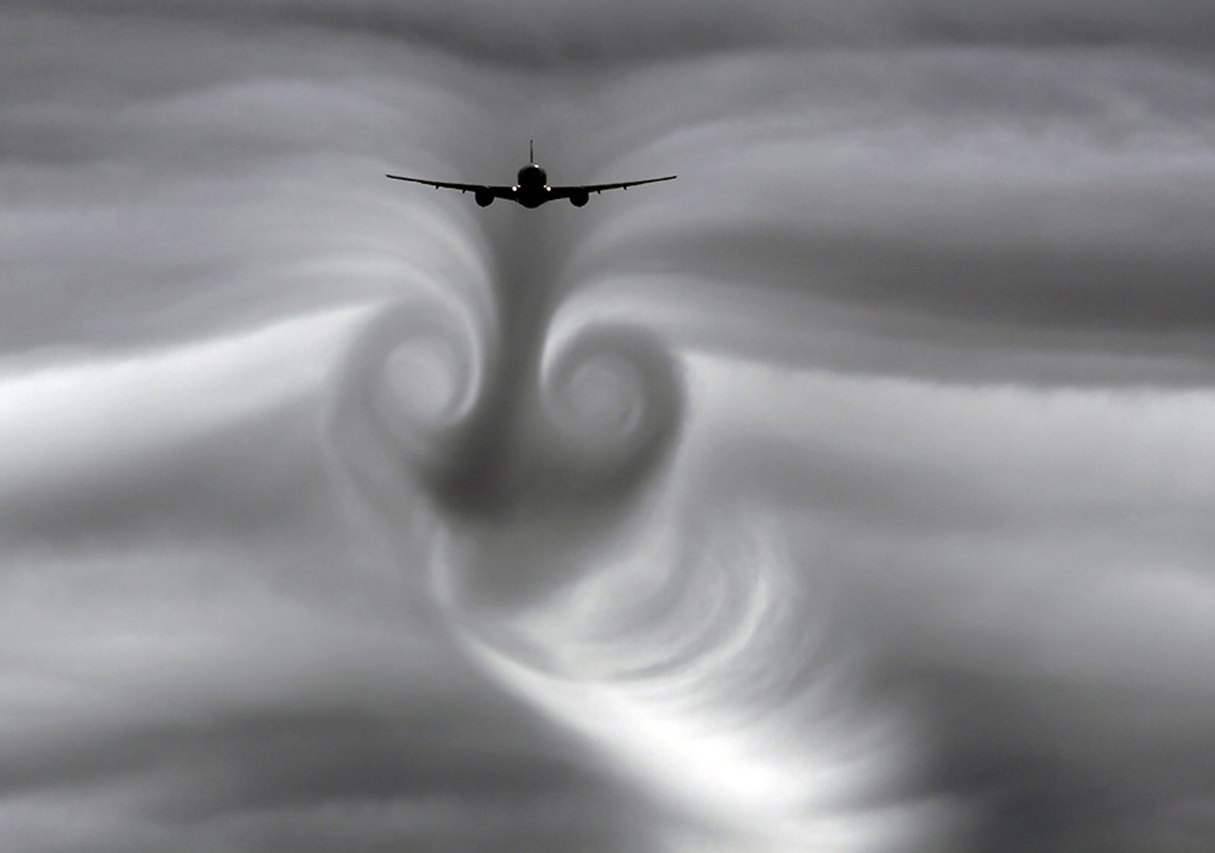
\includegraphics[scale=0.14]{./photo_plane.png}
          \caption{\label{image:plane} Avião em voo, movimentando o ar atmosférico.}
        \end{figure}
      \end{minipage}
		\end{frame}

		\begin{frame}
      \frametitle{Aspectos históricos}
      \begin{minipage}[h!]{0.49\textwidth}
			$\bullet$ Archimedes que desenvolveu as leis da flutuação.\\ 
      $\bullet$ Escola alexandrina onde se desenvolveram bombas hidráulicas sendo também estudadas diversas aplicações de escoamentos confinados.\\
      $\bullet$ Estudiosos islâmicos que desenvolveram pesquisas no campo da hidro-estática.\\
      $\bullet$ Benedetto Castelli, Evangelista Torricelli e Blaise Pascal formalizaram conceitos com seus estudos.\\
      $\bullet$ Isaac Newton, onde ele descreve fluidos incompressíveis e as forças viscosas que afetam seu movimento a baixos números de Reynolds.\\
      $\bullet$ Daniel Bernoulli. Ele estudou a transformação de energia da velocidade dos fluidos em pressão

      \end{minipage}
      \begin{minipage}[h!]{0.49\textwidth}
        \begin{figure}[h!]
          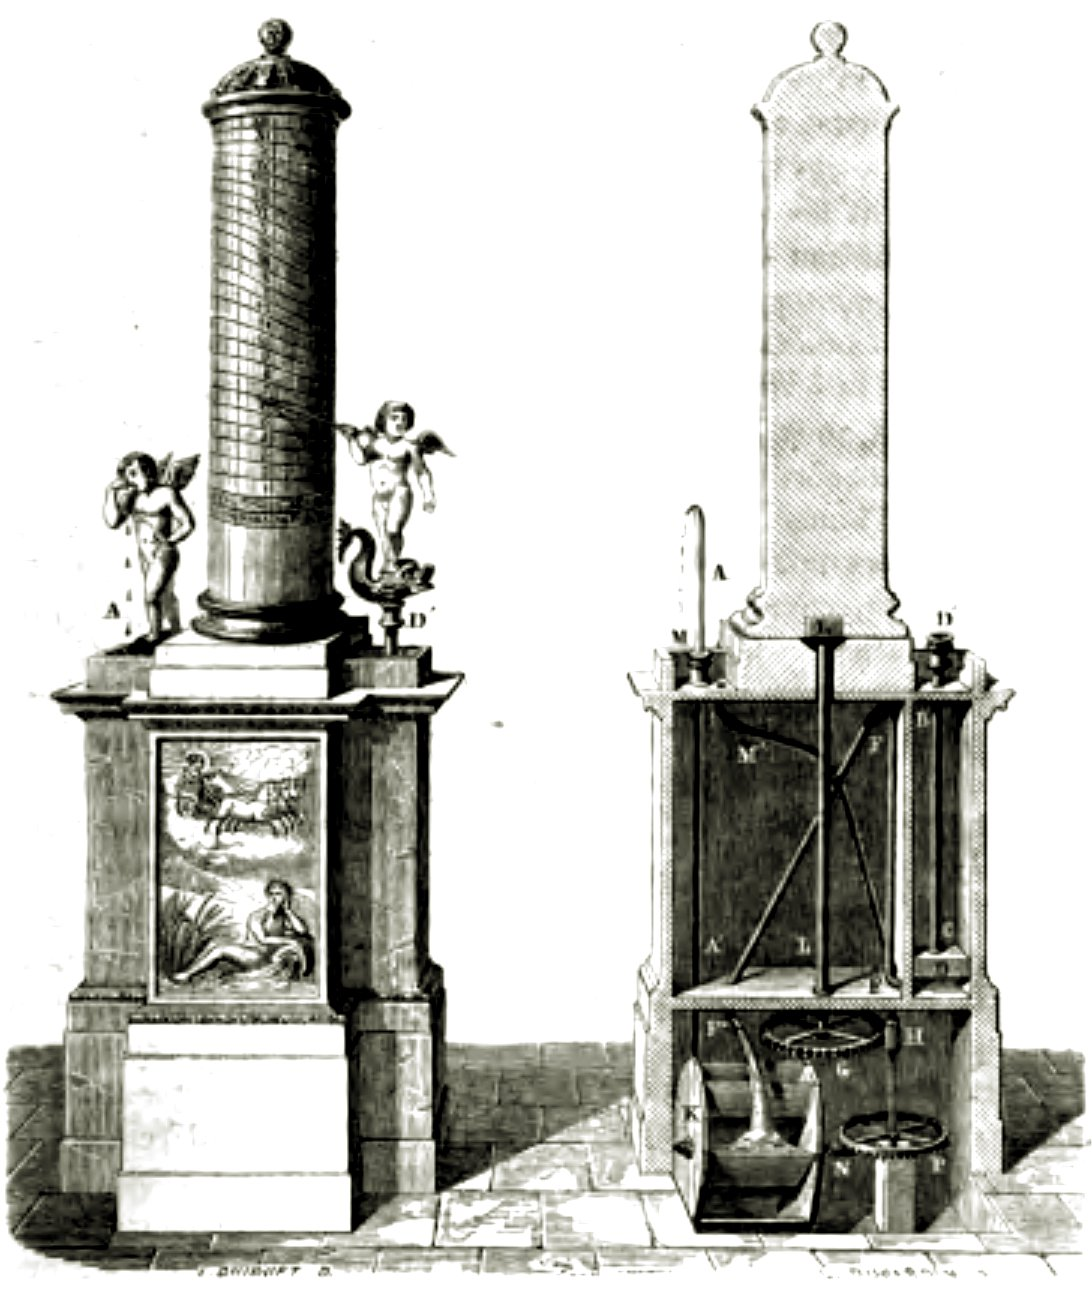
\includegraphics[scale=0.07]{ctesibius.jpeg}
          \caption{\label{image:ctesibius} Relógio de água de Ctesibius, visualização criada pelo arquiteto francês Claude Perrault}
        \end{figure}
      \end{minipage}
		\end{frame}

		\begin{frame}
      \frametitle{Aspectos históricos}
      Tais estudos acadêmicos culminaram com os estudos de  Claude-Louis Navier e George Gabriel Stokes, que desenvolveram as equações de Navier-Stokes:

      \begin{equation}
      \rho \vec{g}-\nabla \vec{p}+\eta \cdot \nabla^{2} \vec{u}=\rho \cdot\left(\vec{u} \cdot \nabla \vec{u}+\frac{\partial \vec{u}}{\partial t}\right)
      \end{equation}

      Sem solução analítica geral, as equações de Navier-Stokes são resolvidas numericamente para casos específicos. É possível, também, a partir de simplificações e ajustes, desconsiderar alguns termos de forma a se conseguir soluções contínuas para casos suficientemente simples.

      Um exemplo de sistema simplificado é o escoamento de Poiseuille. Descrito com a equação que segue:

      \begin{equation}
        u(y) = \frac{G}{2\mu}y (h - y).
      \end{equation}

      Onde G é um gradiente de pressão constante no sentido da corrente ($G = -\frac{dp}{dx}$), e $\mu$ é o coeficiente de viscosidade. Para casos não laminares, ou seja, em que o fluido se movimenta não só na direção principal, essa equação já se distancia da realidade.
		\end{frame}





	\section{Modelo físico}
	
	
	
	
	
		\begin{frame}
			\frametitle{Escoamento de Poiseuille plano}
			$\bullet$ Um escoamento de canal, com somente uma dimensão finita no eixo $y$. \\
			$\bullet$ Condições de contorno de duas placas planas infinitas em um regime de fluxo térmico constante.\\
			$\bullet$ Gradiente de pressão constante no eixo $x$.\\
			$\bullet$ Auto similaridade dinâmica e térmica no eixo $z$. \\
			$\bullet$ Escoamento incompressível, composto por fluido Newtoniano e em regime turbulento.\\
			\begin{minipage}[h!]{0.3\textwidth}
				\begin{equation*}
				 \frac{\partial T }{\partial z} = 0.
				\end{equation*}
				\begin{equation*}
				\frac{\partial \overline{u} }{\partial z} = 0.
				\end{equation*}
				\begin{equation*}
				\frac{\partial u }{\partial x} = 0.
				\end{equation*}
      \end{minipage}
      \begin{minipage}[h!]{0.5\textwidth}
        \begin{figure}[h!]
          \centering
          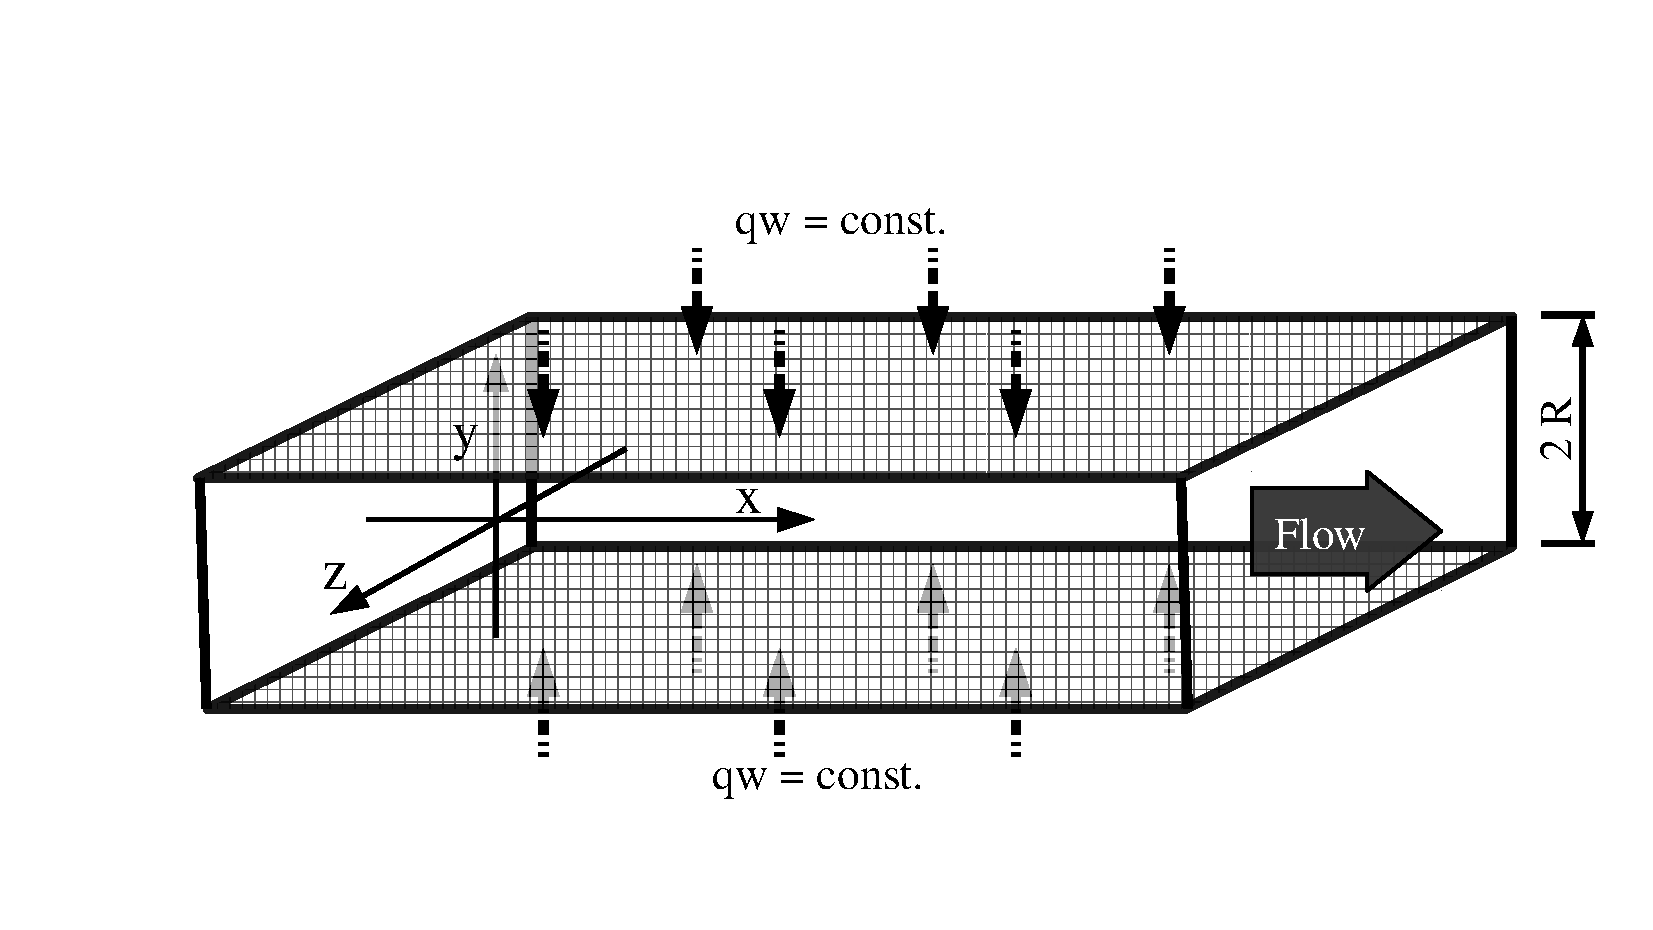
\includegraphics[angle=0, trim={0mm 23mm 0mm 35mm}, clip , scale=0.42]{cap_fundamentacao/canal1.pdf}
          \caption{Definição geométrica e condições de contorno.}
          \label{descricaoGeometrica}
        \end{figure}
			\end{minipage}
			\\
		\end{frame}

		\begin{frame}
			\frametitle{Perfil térmico e dinâmico esperado}
      $\bullet$ A velocidade média é constante em $x$ e no tempo.\\
      $\bullet$ A temperatura média aumenta com $x$ e com o tempo.\\
      \begin{figure}[h!]
        \centering
        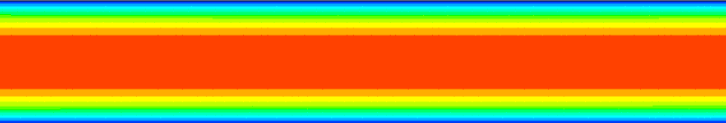
\includegraphics[angle=0, height=1.35cm , width=12.3cm]{cap_fundamentacao/velocidade.png}
        \caption{Campo de velocidade média no canal de Poiseuille. O perfil se mantém constante na direção do escoamento.}
        \label{figure.3}
      \begin{figure}[h!]
        \centering
        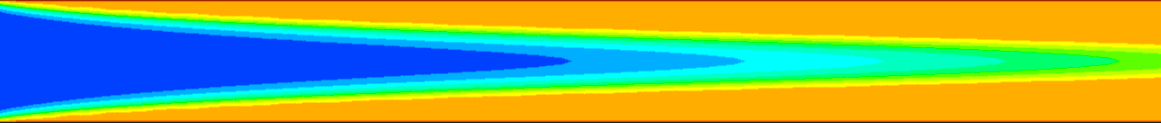
\includegraphics[angle=0, scale=0.4]{cap_fundamentacao/temperatura.png}
        \caption{Campo de temperatura média no canal de Poiseuille. O perfil de temperatura no canal aumenta linearmente na direção do escoamento.}
        \label{figure.2}
      \end{figure}
      \end{figure}
		\end{frame}
	
	

	
	\section{Modelo matemático diferencial}
	
	
	
	
		
		\begin{frame}
		\frametitle{Equações do movimento}
		A equação da continuidade e a equação de Navier-Stokes para a velocidade no eixo de interesse são importantes nesse estágio.
		\begin{equation}
		\frac{\partial u}{\partial t} + \frac{\partial u^2}{\partial x} + \frac{\partial uv}{\partial y} + \frac{\partial uw}{\partial z} = - \frac{1}{\rho} \frac{\partial {p}}{\partial x} + \nu \left( \frac{\partial^2 u}{\partial x^2} + \frac{\partial^2 u}{\partial y^2} + \frac{\partial^2 u}{\partial z^2}   \right)
		\end{equation}
		\begin{equation}
		\frac{\partial \rho}{\partial t} +  \frac{\partial (\rho u)}{\partial x} + \frac{\partial (\rho v)}{\partial y} + \frac{\partial (\rho w)}{\partial z} = 0
		\end{equation}
    Uma vez que tem-se um contexto convectivo, o perfil de velocidade é necessário para a resolução das equações.
		\end{frame}

		



		\begin{frame}
      \frametitle{Equação do balanço da energia térmica}
      Foi utilizada a equação da energia térmica.
      \begin{equation}
      \frac{\partial T}{\partial t} + {\frac{\partial{}}{\partial{x}} (uT)} + {\frac{\partial{}}{\partial{y}} (vT)} + {\frac{\partial{}}{\partial{z}} (wT)}
      =
      {\frac{\partial{}}{\partial{x}}} \left(\alpha {\frac{\partial{T}}{\partial{x}}} \right) +
      {\frac{\partial{}}{\partial{y}}} \left(\alpha {\frac{\partial{T}}{\partial{y}}} \right) +
      {\frac{\partial{}}{\partial{z}}} \left(\alpha {\frac{\partial{T}}{\partial{z}}} \right) .
      \end{equation}
      $ $
      Também foi realizado um balanço de energia térmica a título de adimensionalização:
      \begin{equation}\label{c_h_e}
      q_{conv.} = \dot{m} C_p \Delta T_m.
      \end{equation}
      $ $
		\end{frame}




		
		
		\begin{frame}
			\frametitle{Tratamento estatístico das equações}
			Para se prosseguir com as simplificações das equações diferenciais foi necessário se utilizar os conceitos de valores médios. Tal consideração implica no uso do modelo RANS. (Reynolds Averaged Navier Stokes)
			\\
			\begin{minipage}[h!]{0.45\textwidth}
				\begin{equation*}
				\label{ola}
				\text{Simplificação}=
				\begin{cases}
				\overline{f}({x})=\frac{1}{t_f - t_i} \int_{t_i}^{t_f} f({x} , t) dt.      & \quad  \\
				f({x} , t) = \overline{f}({x}) + f^\prime ({x} ,t) . & \quad   \\
				\overline{f^\prime ({x} ,t)} = 0 . & \quad   \\
				\overline{\overline{f({x})}} = \overline{f({x})} . & \quad   \\
				\overline{f^\prime ({x} ,t)\overline{f({x})}} = 0 .& \quad   \\
				\overline{f^\prime ({x} ,t)g^\prime ({x} ,t)} \neq 0 . & \quad   \\
				\overline{  \overline{g({x})} \ \overline{f({x})}  } = {\overline{g({x})}} \ {\overline{f({x})}} . & \quad   \\
				\end{cases}
				\end{equation*}
			\end{minipage}\hfill
			\begin{minipage}[h!]{0.45\textwidth}
				\begin{figure}
					\centering
					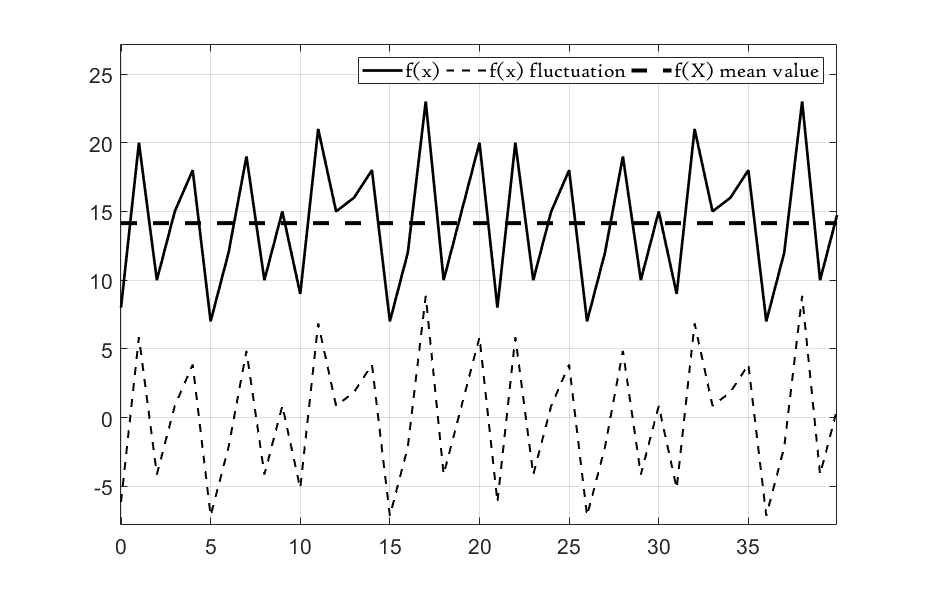
\includegraphics[angle=0, scale=0.3]{medios}
					\caption{Representação gráfica do conceito.}
					\label{medios}
				\end{figure}
			\end{minipage}
	     	\\
		\end{frame}
	
	
	
	
	
		
				\begin{frame}
		\frametitle{Simplificando a velocidade para valores médios}
		\begin{equation}
		\frac{\partial \overline{u}}{\partial t} + \frac{\partial \overline{u^2}}{\partial x} + \frac{\partial \overline{uv}}{\partial y} + \frac{\partial \overline{uw}}{\partial z} = - \frac{1}{\rho}  \frac{\partial \overline{p}}{\partial x} + \nu  \left( \frac{\partial^2 \overline{u}}{\partial {x^2}} + \frac{\partial^2 \overline{u}}{\partial y^2} + \frac{\partial^2 \overline{u}}{\partial z^2}   \right)
		\end{equation}
		\\
		\begin{equation}
		\begin{split}
		\frac{\partial \overline{(\overline{u} + u^\prime)}}{\partial t} + \frac{\partial \overline{(\overline{u}^2 + 2  \overline{u}  u^\prime + {u^\prime}^2)}}{\partial x} + \frac{\partial \overline{(\overline{u}\ \overline{v} + u^\prime  \  \overline{v} + \overline{u}  v^\prime + u^\prime  v ^\prime )}}{\partial y} + \\
		\frac{\partial \overline{(\overline{u} \ \overline{w} + u^\prime  \overline{w} + \overline{u}  w^\prime + u^\prime  w ^\prime )}}{\partial z} = - \frac{1}{\rho}  \frac{\partial \overline{(\overline{p} + p ^\prime)}}{\partial x} + \nu  \left( \frac{\partial^2 \overline{(\overline{u} + u^\prime)}}{\partial {x^2}} + \frac{\partial^2 \overline{(\overline{u} + u^\prime)}}{\partial y^2} + \frac{\partial^2 \overline{(\overline{u} + u^\prime)}}{\partial z^2}   \right)
		\end{split}
		\end{equation}
		\\
		\begin{equation}
		\begin{split}
		\frac{\partial \overline{u}}{\partial t} + \frac{\partial \overline{u^2}}{\partial x} + \frac{\partial \overline{u} \ \overline{v}}{\partial y} + \frac{\partial \overline{u} \ \overline{w}}{\partial z} =  - \frac{1}{\rho}  \frac{\partial \overline{{p}}}{\partial x} + \frac{\partial}{\partial x} \left( \nu \frac{\partial \overline{u}}{\partial x} - \overline{{u^\prime}^2}\right) + \frac{\partial}{\partial y} \left( \nu \frac{\partial \overline{u}}{\partial y} - \overline{{u^\prime v^\prime}}\right) \\
		+ \frac{\partial}{\partial z} \left( \nu  \frac{\partial \overline{u}}{\partial z} - \overline{ u ^\prime w ^\prime} \right)
		\end{split}
		\end{equation}
		\end{frame}
		
		
		
		
		
		\begin{frame}
			\frametitle{Simplificando a equação da continuidade para valores médios}
			Desenvolvendo a equação da Continuidade, tem-se:
			\begin{equation*}
			\frac{\partial \rho}{\partial t} +  \frac{\partial (\rho u)}{\partial x} + \frac{\partial ( \rho v)}{\partial y} + \frac{\partial (\rho w)}{\partial z} = 0
			\end{equation*}
			\begin{equation}
			\frac{\partial u}{\partial x} + \frac{\partial v}{\partial y} + \frac{\partial w}{\partial z} = 0
			\end{equation}
			\begin{equation}
			\frac{\partial \overline{(u^\prime + \overline{u})}}{\partial x} + \frac{\partial \overline{(v^\prime + \overline{v})}}{\partial y} + \frac{\partial \overline{(w^\prime + \overline{w})}}{\partial z} = 0
			\end{equation}
			\begin{equation}
			\frac{\partial \overline{u^\prime}}{\partial x} +\frac{\partial \overline{\overline{u}}}{\partial x} + \frac{\partial \overline{v\prime}}{\partial y} +\frac{\partial \overline{\overline{v}}}{\partial y} + \frac{\partial \overline{w\prime}}{\partial z} +\frac{\partial \overline{\overline{w}}}{\partial z} = 0
			\end{equation}
			\begin{equation}
			\frac{\partial {\overline{u}}}{\partial x} +\frac{\partial {\overline{v}}}{\partial y} +\frac{\partial {\overline{w}}}{\partial z} = 0
			\end{equation}
			Assim, como $ \frac{\partial {\overline{v}}}{\partial y} $ e $ \frac{\partial {\overline{w}}}{\partial z}$ são iguais a zero, por definição do comportamento médio dos escoamentos, necessariamente $\frac{\partial {\overline{u}}}{\partial x}$ deve ser igual a zero também, o que demonstra como o sistema resultante é unidimensional.
		\end{frame}
		
		
		
		
		\begin{frame}
		\frametitle{Simplificando a temperatura para valores médios}
		\begin{equation}
		\frac{\partial \overline{T}}{\partial t} + {\frac{\partial{}}{\partial{x}} \overline{(u T)}} + 
		{\frac{\partial{}}{\partial{y}} \overline{(v T)}} 
		=
		{\frac{\partial{}}{\partial{x}}} \left(\alpha {\frac{\partial{\overline{T}}}{\partial{x}}} \right) +
		{\frac{\partial{}}{\partial{y}}} \left(\alpha {\frac{\partial{\overline{T}}}{\partial{y}}} \right) .
		\end{equation}
		\begin{equation}
		\begin{split}
		\frac{\partial \overline{(\overline{T} + T^\prime)}}{\partial t} +{\frac{\partial{}}{\partial{x}} \overline{\left((\overline{u} + u^\prime)  (\overline{T} + T^\prime) \right)}} + 
		{\frac{\partial{}}{\partial{y}} \overline{(\left(\overline{v} + v^\prime)  (\overline{T} + T^\prime) \right)}} 
		= \\
		{\frac{\partial{}}{\partial{x}}} \left(\alpha {\frac{\partial{\overline{(\overline{T} + T^\prime)}}}{\partial{x}}} \right) +
		{\frac{\partial{}}{\partial{y}}} \left(\alpha {\frac{\partial{\overline{(\overline{T} + T^\prime)}}}{\partial{y}}} \right) .
		\end{split}
		\end{equation}
		\begin{equation}
		\frac{\partial \overline{T}}{\partial t} +\frac{\partial{}}{\partial{x}} \left(\overline{\left({T^\prime u^\prime}\right)} + \overline{u} \ \overline{T}\right)     + 
		\frac{\partial{}}{\partial{y}} \left(\overline{\left({T^\prime v^\prime}\right)} + \overline{v} \ \overline{T}\right) 
		=
		{\frac{\partial{}}{\partial{x}}} \left(\alpha {\frac{\partial{\overline{T}}}{\partial{x}}} \right) +
		{\frac{\partial{}}{\partial{y}}} \left(\alpha {\frac{\partial{\overline{T}}}{\partial{y}}} \right) .
		\end{equation}
		\begin{equation}\label{equation_preparede}
		\frac{\partial \overline{T}}{\partial t} +\frac{\partial{}}{\partial{x}} \left(\overline{T^\prime  u^\prime}\right) + \frac{\partial{}}{\partial{x}}\left(\overline{u} \ \overline{T}\right)     + 
		\frac{\partial{}}{\partial{y}} \left(\overline{T^\prime v^\prime}\right) + \frac{\partial{}}{\partial{x}}\left(\overline{v} \ \overline{T}\right) 
		=
		{\frac{\partial{}}{\partial{x}}} \left(\alpha {\frac{\partial{\overline{T}}}{\partial{x}}} \right) +
		{\frac{\partial{}}{\partial{y}}} \left(\alpha {\frac{\partial{\overline{T}}}{\partial{y}}} \right) .
		\end{equation}
		\end{frame}
		
		
	
	
	
		\begin{frame}
		\frametitle{Balanço de energia}
		Apesar de já estar em valores médios, a temperatura no domínio não reduz a um problema unidimensional:
		\begin{equation}\label{c_h_e}
		q_{conv.} = \dot{m} C_p \Delta T_m.
		\end{equation}
		\begin{equation}
		2q_w b \Delta x = \dot{m} C_p \Delta T_m.
		\end{equation}
		Sendo $b$ a profundidade do canal e $T_m$ a temperatura média em uma secção transversal. Então, substituindo $ \dot{m} = u_m 2R b \rho $, e considerando $ \Delta T_m = \frac{\partial{\left(\overline{T}_m\right)}}{\partial{x}} \Delta x $:
		\begin{equation}
		2q_w b \Delta x = u_m 2R b \rho  C_p \frac{\partial{\left(\overline{T}_m\right)}}{\partial{x}} \Delta x.
		\end{equation}     
		\begin{equation}
		q_w = u_m R \rho  C_p \frac{\partial{\left(\overline{T}_m\right)}}{\partial{x}} .
		\end{equation} 
		\begin{equation}\label{c_h_ee}
		\frac{\partial{\left(\overline{T}_m\right)}}{\partial{x}} = \frac{q_w}{u_m  R \rho  C_p } .
		\end{equation} 
		\end{frame}
	
	
	
	
		\begin{frame}
		\frametitle{Análise da temperatura de parede}
		Para esta análise empregou-se um estudo do fluxo térmico convectivo, que pode ser expresso matematicamente por:
		\begin{equation}
		q_w = h A \left( T_w(x) - \overline{T}_m(x)\right).
		\end{equation}
		Nota-se que $h$ é constante, pois tem-se um escoamento completamente desenvolvido. Assim é possível escrever:
		\begin{equation}
		 T_w(x) - \overline{T}_m(x) = \frac{q_w}{hA}.
		\end{equation}
		\begin{equation}
		\frac{d T_w(x)}{d x} - \frac{d \overline{T}_m(x)}{d x} = \frac{d \frac{q_w}{hA}}{dx}.
		\end{equation}
		\begin{equation}
		\frac{d T_w(x)}{d x} = \frac{d \overline{T}_m(x)}{d x} = Ctt.
		\end{equation}	
		\end{frame}
	
	
	
	
		\begin{frame}
			\frametitle{Diferença de temperatura}
			Tem-se um gradiente linear de temperatura nas paredes no sentido do eixo $x$. Para que se obtenha um fluxo térmico constante no canal.  \\
			\begin{minipage}[h!]{0.36\textwidth}
				\begin{equation}
				\frac{\partial \overline{T}}{\partial x} = ctt.
				\end{equation}
				Dessa forma, para se ter um sistema unidimensional representativo, se parametrizou a variável em função da temperatura na parede, ou seja:
				\begin{equation}
				\overline{T}^\ast(y) = \overline{T}(x,y)  - \overline{T}_w(x) .
				\end{equation}
				\begin{equation}
				\overline{T}(x,y) = \overline{T}^\ast(y) + \overline{T}_w(x).
				\end{equation}
			\end{minipage}\hfill
			\begin{minipage}[h!]{0.60\textwidth}
			\begin{figure}
				\centering
				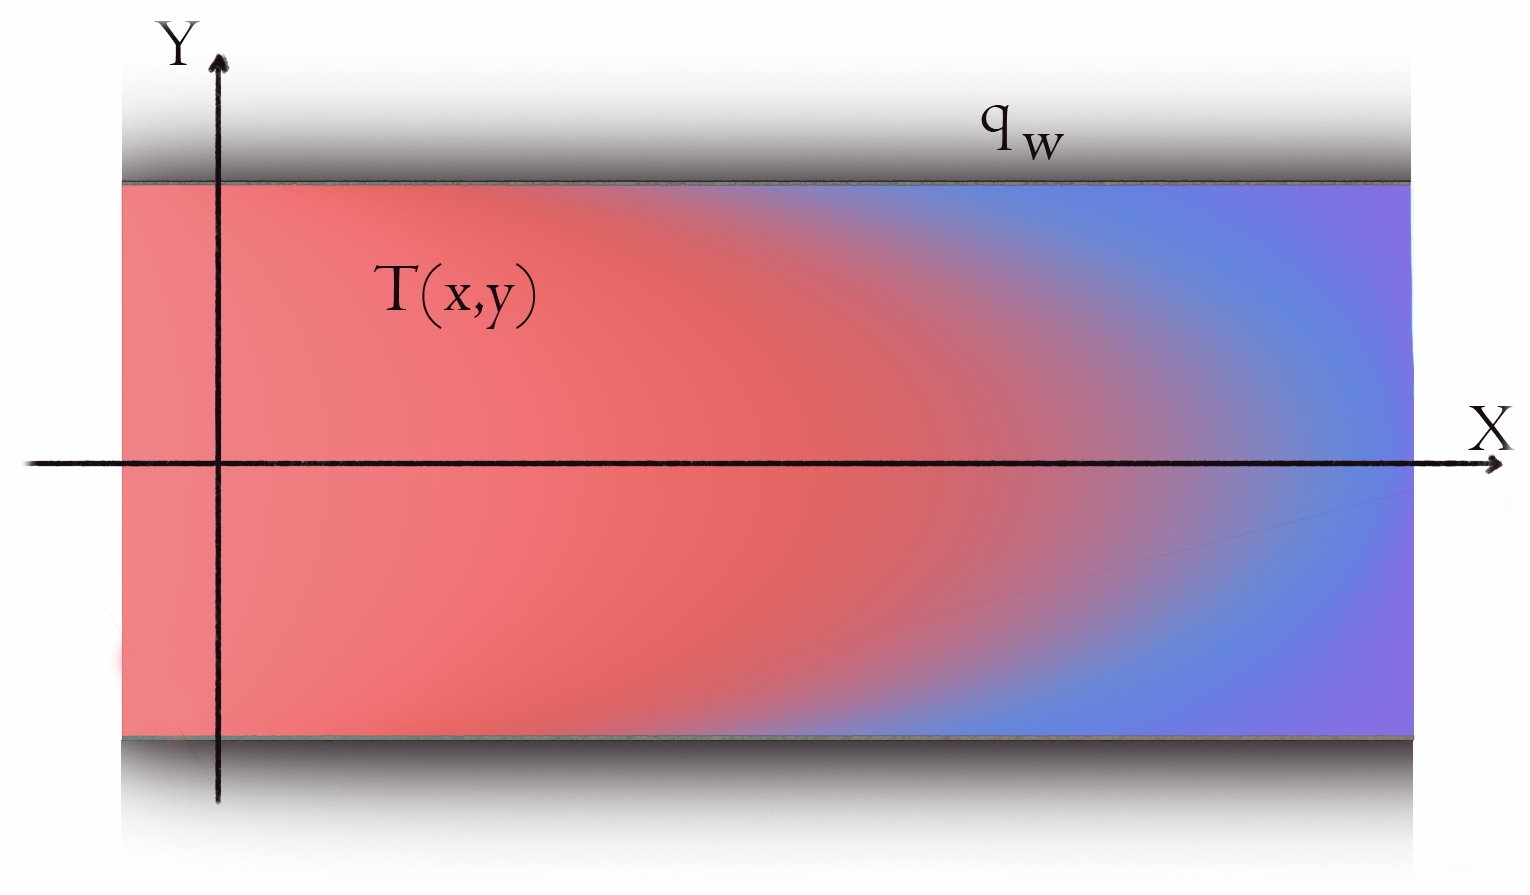
\includegraphics[angle=0, scale=0.14]{imagemtermico}
				\caption{Representação gráfica do domínio térmico do sistema.}
				\label{temperatura}
			\end{figure}
			\end{minipage}
		\end{frame}
		
		
		
		
		
		
		\begin{frame}
		\frametitle{Desenvolvendo a diferença de temperatura na equação}
		\begin{equation}
		\begin{split}
		\frac{\partial ( \overline{T^\ast + T_w}  ) }{\partial t} +
		\frac{\partial{}}{\partial{x}} \left(\overline{(T^\ast + T_w)^\prime u^\prime}\right) + \frac{\partial{}}{\partial{x}}\left(\overline{(T^\ast + T_w)} \ \overline{u}\right)+  \\
		\frac{\partial{}}{\partial{y}} \left(\overline{(T^\ast + T_w)^\prime v^\prime}\right) + \frac{\partial{}}{\partial{y}}\left(\overline{(T^\ast + T_w)} \ \overline{v}\right) = \\
		{\frac{\partial{}}{\partial{x}}} \left(\alpha {\frac{\partial{\overline{(T^\ast + T_w)}}}{\partial{x}}} \right) +
		{\frac{\partial{}}{\partial{y}}} \left(\alpha {\frac{\partial{\overline{(T^\ast + T_w)}}}{\partial{y}}} \right) .
		\end{split}
		\end{equation}
		\begin{center}\begin{equation}\begin{split}
		\frac{\partial ( \overline{ T^\ast + T_w } ) }{\partial t} +
		\frac{\partial{}}{\partial{x}} \left(\overline{T_w^{\prime} u^{\prime}}\right) +\frac{\partial{}}{\partial{x}} \left(\overline{{T^{\ast}}^{\prime} u^{\prime}}\right)
		+\frac{\partial{}}{\partial{x}}\left(\overline{u} \ \overline{T^{\ast}}\right)+ 
		\frac{\partial{}}{\partial{x}}\left(\overline{u} \ \overline{T_w}\right)+ 
		\\
		\frac{\partial{}}{\partial{y}} \left(\overline{{T^{\ast}}^{\prime} v^{\prime}}\right)+
		\frac{\partial{}}{\partial{y}} \left(\overline{T_w^\prime v^\prime}\right) + \frac{\partial{}}{\partial{y}}\left(\overline{v} \ \overline{T^\ast}\right) +
		\frac{\partial{}}{\partial{y}}\left(\overline{v} \ \overline{T_w}\right) 
		= 
		\\
		{\frac{\partial{}}{\partial{x}}} \left(\alpha {\frac{\partial{\overline{(T^\ast + T_w)}}}{\partial{x}}} \right) +
		{\frac{\partial{}}{\partial{y}}} \left(\alpha {\frac{\partial{\overline{(T^\ast + T_w)}}}{\partial{y}}} \right) .
		\end{split}\end{equation}\end{center}
		\end{frame}
		
		
		
		
		
		\begin{frame}
			\frametitle{Equação dinâmica simplificada}
			Para a velocidade, devem ser feitas as considerações de que é um sistema em regime permanente e unidimensional.
			Assim, na equação da velocidade, teremos as seguintes simplificações:
			\begin{equation}
			\begin{split}
			\frac{\partial \overline{u}}{\partial t} + \frac{\partial \overline{u^2}}{\partial x} + \frac{\partial \overline{u} \ \overline{v}}{\partial y} +  \frac{\partial \overline{u} \ \overline{w}}{\partial z}  =  - \frac{1}{\rho} \frac{\partial \overline{{p}}}{\partial x} + \frac{\partial}{\partial x} \left( \nu \frac{\partial \overline{u}}{\partial x} - \overline{{u^\prime}^2}\right) + \frac{\partial}{\partial y} \left( \nu \frac{\partial \overline{u}}{\partial y} - \overline{{u^\prime  v^\prime}}\right) \\
			+ \frac{\partial}{\partial z} \left( \nu  \frac{\partial \overline{u}}{\partial z} - \overline{ u ^\prime w ^\prime} \right)
			\end{split}
			\end{equation}
			\begin{equation}
			\frac{1}{\rho} \frac{\partial \overline{p}}{\partial x} = \frac{\partial}{\partial y} \left( \nu \frac{\partial \overline{u}}{\partial y} - \overline{u^\prime v^\prime}\right)  
			\end{equation}
		\end{frame}
		
		
		
		
		
		\begin{frame}
		\frametitle{Equação térmica simplificada}
		Para a temperatura, foi considerado um regime permanente, derivadas nulas quanto à temperatura e diferença de temperatura, além de que considerou-se a temperatura de parede estável, ou seja, sem flutuações. 
	 	\begin{center}
	 	\begin{equation*}
	 		\begin{split}
	 		\frac{\partial ( \overline{ T^\ast + T_w } ) }{\partial t}  +
	 		\frac{\partial{}}{\partial{x}} \left(\overline{ T_w^{\prime}  u^{\prime}}\right) +
	 		\frac{\partial{}}{\partial{x}} \left(\overline{{T^{\ast}}^{\prime} u^{\prime}}\right)+ 
	 		 \frac{\partial{}}{\partial{x}}\left(\overline{u} \ \overline{T^{\ast}}\right) + 
	 		\frac{\partial{}}{\partial{x}}\left(\overline{u} \ \overline{T_w}\right)+ 
	 		\\
	 		\frac{\partial{}}{\partial{y}} \left(\overline{{T^{\ast}}^{\prime} v^{\prime}}\right)+
	 		\frac{\partial{}}{\partial{y}} \left(\overline{T_w^\prime  v^\prime}\right) + \frac{\partial{}}{\partial{y}}\left(\overline{v}  \ \overline{T^\ast}\right) +
	 		\frac{\partial{}}{\partial{y}}\left(\overline{v} \ \overline{T_w}\right) 
	 		= 
	 		\\
	 		{\frac{\partial{}}{\partial{x}}} \left(\alpha {\frac{\partial{\overline{(T^\ast + T_w)}}}{\partial{x}}} \right) +
	 		{\frac{\partial{}}{\partial{y}}} \left(\alpha {\frac{\partial{\overline{(T^\ast +  T_w )}}}{\partial{y}}} \right) .
	 		\end{split}
	 	\end{equation*}
 		\end{center}
 		\begin{equation}\label{equation_var}
 			{\frac{\partial{}}{\partial{y}}} \left(\alpha {\frac{\partial{\overline{T^\ast}}}{\partial{y}}}   
 			- \left(\overline{ T^{\ast\prime} v^\prime}\right) \right)
 			= 
 			\overline{u}\frac{\partial{}}{\partial{x}}\left(\overline{T_w}\right)  .
 		\end{equation}
		\end{frame}


		
		\begin{frame}
			\frametitle{Hipótese de Boussinesq}
			O fluxo turbulento ($\overline{T^{\ast\prime}  v^\prime}$) pode ser desenvolvido segundo a hipótese de Boussinesq, que postula:
			\begin{equation}\label{bou}
			-\left(\overline{ u^\prime  v^\prime}\right) = 
			\nu_t \frac{\partial{\overline{u}}}{\partial{y}}
			\implies
			-\left(\overline{ T^{\ast\prime}  v^\prime}\right) = 
			\alpha_t \frac{\partial{\overline{T^\ast}}}{\partial{y}}.
			\end{equation}
			Assim, tem-se: 
			\\
				\begin{equation}
				{\frac{\partial{}}{\partial{y}}} \left(\alpha {\frac{\partial{\overline{T^\ast}}}{\partial{y}}}   
				+ \alpha_t  \frac{\partial \overline{T^\ast}}{\partial y} \right)
				= 
				\overline{u}\frac{\partial{}}{\partial{x}}\left(\overline{T_w}\right) . 
				\end{equation}
		\end{frame}
	
	
	
	
		
		\begin{frame}
			\frametitle{Comprimento de mistura de Prandtl}
			Para modelar a difusidade térmica turbulenta ($\alpha_t$) uma nova variável deve ser introduzida, o número de Prandtl turbulento, como segue:
			\begin{equation}
				Pr_t = \frac{\nu_t}{\alpha_t}.
			\end{equation} 
			O valor do número de Prandtl turbulento de $ Pr_t = 0.71$ tem sido utilizado na literatura, como visto em Turbulence in Fluids (M. Lesieur).
			Para modelar $\nu_\tau$ tem-se o modelo do comprimento de mistura de Prandtl:
			\begin{equation}
			\nu_t = {l_m}^2 \left| \frac{\partial \overline{u}}{\partial y} \right|.
			\end{equation}
		\end{frame}
		
		
		
		
		
		\begin{frame}
			\frametitle{Substituindo o comprimento de mistura na equação principal}	
			O comprimento de mistura introduz um módulo no modelo diferencial e o parâmetro do número de Prandtl turbulento.   
			\\
				\begin{equation}
				{\frac{\partial{}}{\partial{y}}} \left( \left( \alpha   
				+ \frac{\nu_t}{Pr_t} \right) \frac{\partial \overline{T^\ast}}{\partial y} \right)
				= 
				\overline{u}\frac{\partial{}}{\partial{x}}\left(\overline{T_w}\right)  .
				\end{equation}
			\begin{equation}
			{\frac{\partial{}}{\partial{y}}} \left( \left( \alpha   
			+ \frac{{l_m}^2 \left| \frac{\partial \overline{u}}{\partial y} \right|}{Pr_t} \right) \frac{\partial \overline{T^\ast}}{\partial y} \right)
			= 
			\overline{u}\frac{\partial{}}{\partial{x}}\left(\overline{T_w}\right)  .
			\end{equation}
		\\
		Para valores positivos de $ y $, a primeira derivada da velocidade sempre será negativa, visto que pelos princípios de Dirichlet e Neumman, tem-se uma velocidade que diminui com o aumento de $ y $. Assim, temos:\\
			\begin{equation}
			{\frac{\partial{}}{\partial{y}}} \left( \left( \alpha   
			- \frac{{l_m}^2}{Pr_t}\frac{\partial \overline{u}}{\partial y} \right) \frac{\partial \overline{T^\ast}}{\partial y} \right)
			= 
			\overline{u}\frac{\partial{}}{\partial{x}}\left(\overline{T_w}\right)  .
			\end{equation}
		\end{frame}	
	
	
	
	
		\begin{frame}
			\frametitle{Um modelo para o comprimento de mistura de Prandtl}
			Um modelo para $l_m$ deve ser estabelecido. Para tal, se observou os estudos experimentais de Nikuradse, com o qual modelou-se esse parâmetro como segue.
			\begin{equation}
			L\left(\frac{y}{R}\right) = \frac{l_m}{R} = 0.14 - 0.08 \left(\frac{y}{R}\right)^2 - 0.06\left(\frac{y}{R}\right)^4.
			\end{equation}
			Para enriquecer ainda mais o modelo, Cebeci e Bradshaw acrescentaram a função de amortecimento de Van Driest:
			\begin{equation}
			L\left(\frac{y}{R}\right)  = \frac{l_m}{R} = \left(\frac{l_m}{R} = 0.14 - 0.08 \left(\frac{y}{R}\right)^2 - 0.06\left(\frac{y}{R}\right)^4\right)\left\{  1 - e^{[(\tilde{y} - 1) \frac{Re_\tau}{26}]}\right\}.
			\end{equation}
			Assim, tem-se o comprimento de mistura definido por:
			\begin{equation}
			lm = L R.
			\end{equation}
			Sendo $ L $ uma função em $ y $. É importante notar que neste momento foi introduzida a constante de Cebeci, que é o número $ 26 $ que divide o $ Re_\tau $.
		\end{frame}
		
		
		
		
		
		\begin{frame}
			\frametitle{Substituindo o comprimento de mistura nas equações}
			A função $ L(\frac{y}{R}) $ já está Adimensionalizada. Mas ela pode ser introduzida na equação da temperatura como segue:
				\begin{equation}
				{\frac{\partial{}}{\partial{y}}} \left( \left( \alpha   
				- \frac{{L}^2 R ^2}{Pr_t}\frac{\partial \overline{u}}{\partial y} \right) \frac{\partial \overline{T^\ast}}{\partial y} \right)
				= 
				\overline{u}\frac{\partial{}\left(\overline{T_w}\right)  }{\partial{x}}.
				\end{equation}
		\end{frame}
		
		
		
		
		
		\begin{frame}
			\frametitle{Desenvolvendo a equação dinâmica}
			
			\begin{equation}
			\int \frac{1}{\rho} \frac{\partial \overline{p}}{\partial x} dy = \int \frac{\partial}{\partial y} \left( \nu  \frac{\partial \overline{u}}{\partial y} - {L}^2 R ^2 \left(\frac{\partial \overline{u}}{\partial y}\right) ^ 2 \right) dy  
			\end{equation}
			\begin{equation}
			\frac{1}{\rho} \frac{\partial \overline{p}}{\partial x} \int 1 dy = \int \frac{\partial}{\partial y} \left( \nu  \frac{\partial \overline{u}}{\partial y} - {L}^2 R ^2 \left(\frac{\partial \overline{u}}{\partial y}\right) ^ 2 \right) dy  
			\end{equation}
			\begin{equation}
			y \frac{1}{\rho} \frac{\partial \overline{p}}{\partial x} =  \nu  \frac{\partial \overline{u}}{\partial y} - {L}^2 R ^2 \left(\frac{\partial \overline{u}}{\partial y}\right) ^ 2 
			\end{equation}
			\begin{equation}
			{L}^2 R ^2 \left(\frac{\partial \overline{u}}{\partial y}\right) ^ 2 - \nu  \frac{\partial \overline{u}}{\partial y} + y \frac{1}{\rho} \frac{\partial \overline{p}}{\partial x} = 0
			\end{equation}
			Observando-se a conformação em forma de polinômio de segundo grau, retirou-se as raízes, onde só uma delas teve consistência física.
			\begin{equation}
			\frac{\partial \overline{u}}{\partial y} = \frac{2 y \frac{1}{\rho}\frac{\partial \overline{p}}{\partial x} }{ \nu + \sqrt{\nu ^2 + 4 y \frac{1}{\rho} \frac{\partial \overline{p}}{\partial x} L ^2 R ^2}}
			\end{equation}
		\end{frame}
			
		
		
		
		% \begin{frame}
		% \frametitle{Modelo referente ao gradiente de pressão}
		% Utilizou-se a definição da tenção cisalhante e uma análise segundo a primeira lei de Newton.
		% \begin{equation}
		% u_\tau = \sqrt{\frac{\left| \tau_w \right|}{\rho}}
		% \end{equation}
		% \begin{equation}
		% p_1 2R = 2 \tau_w \Delta x + p_2 2 R
		% \end{equation}
		% Assim, desenvolvendo e substituindo, temos:
		% \begin{equation}
		% \frac{\tau_w}{R} = \frac{(p_1 - p_2)}{\Delta x}
		% \end{equation}
		% \begin{equation}
		% - \frac{\partial \overline{p}}{\partial x} = \frac{\tau_w}{R} = \frac{u_\tau^2 \rho}{R} 
		% \end{equation}
		% \end{frame}
	
	
	
	
	
	
		\begin{frame}
			\frametitle{Adimensionalização}
			Para se comparar mais facilmente os modelos à literatura, adimensionalizou-se as equações segundo coordenadas de parede. Foi considerado: $ \tilde{y} = \frac{y . Re_\tau}{R} $, $ \tilde{\overline{u}} = \frac{\overline{u}}{u_\tau} $ , $ \tilde{\overline{T}} = \frac{\overline{T}}{T_\tau} $ , $Re_\tau = \frac{u_\tau R}{\nu}$, $Pr_t = \frac{\nu_t}{\alpha_t}$, $Pr = \frac{\nu}{\alpha}$ e $T_\tau = \frac{q_w}{\rho C_p u_\tau}$, $\frac{\partial{\left(T_m\right)}}{\partial{x}} = \frac{q_w}{u_m  R \rho  C_p } $, $\frac{\partial \overline{p}}{\partial x} = - \frac{u_\tau^2 \rho}{R} $.
			\\
				\begin{equation}
				{\frac{\partial{}}{\partial{\tilde{y}}}} \left( \left( \frac{Re_\tau}{Pr}   
				- \frac{{L}^2 Re_\tau ^3}{Pr_t}\frac{\partial \tilde{\overline{u}}}{\partial \tilde{y}} \right) \frac{\partial \tilde{\overline{T^\ast}}}{\partial \tilde{y}} \right)
				= 
				\frac{\tilde{\overline{u}}}{\tilde{u_m}}.
				\end{equation}

				\begin{equation}
				\frac{\partial \tilde{\overline{u}}}{\partial \tilde{y}} = - \frac{2 \tilde{y} \frac{1}{Re_\tau} }{ 1 + \sqrt{ 1 + 4 L ^2 Re_\tau ^2 \tilde{y}}}.
				\end{equation}	
				
			Dessa forma, tem-se a primeira derivada da velocidade de forma exata.
		\end{frame}
	
	
	

	
	
	\section{Modelo numérico}
		
	
	
	
		
		\begin{frame}
			\frametitle{Discretização do espaço}
			\begin{minipage}[h!]{0.39\textwidth}
      No modelo numérico se utilizou:\\
        $\bullet$ Domínio Euleriano.\\
        $\bullet$ Método Runge-Kutta de quarta ordem para o domínio dinâmico.\\
        $\bullet$ diferenças centradas para o domínio térmico resolvido de forma implicita.\\
        $\bullet$ Paredes em centro de célula.\\
      Resultados de convergência podem ser vistos na imagem.
			\end{minipage}\hfill
			\begin{minipage}[h!]{0.60\textwidth}
      \begin{figure}[!h]
        \centering
        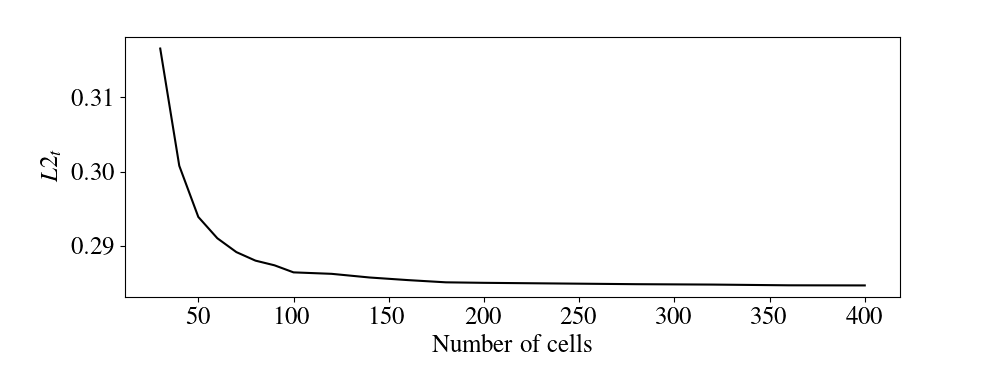
\includegraphics[angle=0, trim={10mm 0mm 0mm 0mm}, clip , scale=0.40]{fotos_formatacao_final/Convergence}
        \caption{Norma L2 de simulação térmica comparado a DNS até 400 células, com $Re_\tau = 1020$.}
      \end{figure}

			\end{minipage}\\
		\end{frame}
	
	
	
	
	
  \begin{frame}
    \begin{figure}
      \centering
      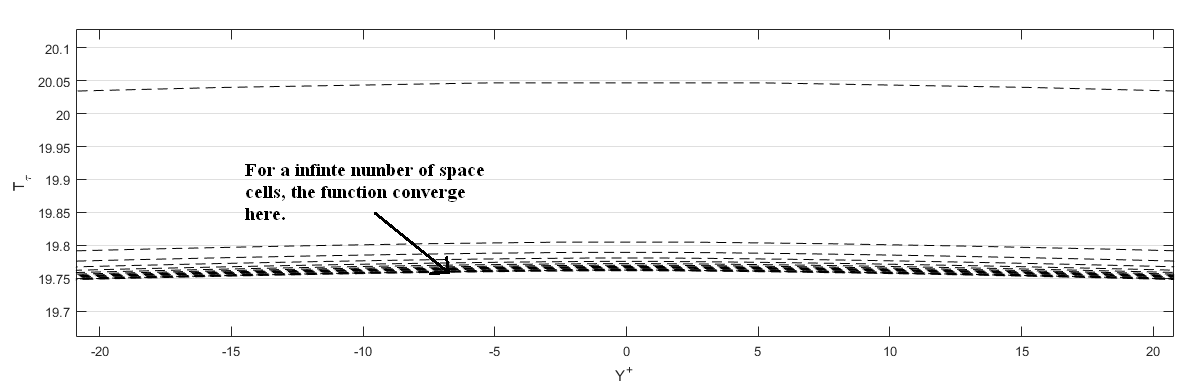
\includegraphics[angle=0, scale=0.42]{convergnciaprimeira}
      \caption{Convergência e independência de malha.}
      \label{convergencia}
    \end{figure}
  \end{frame}


	
	

	\section{Resultados}
  \begin{frame}
    \frametitle{Resultados para: $Pr_t= 0.71$ , $A = 26 $}
    \begin{figure}[!h]
        \centering
        \begin{minipage}{0.49\textwidth}
          \centering
          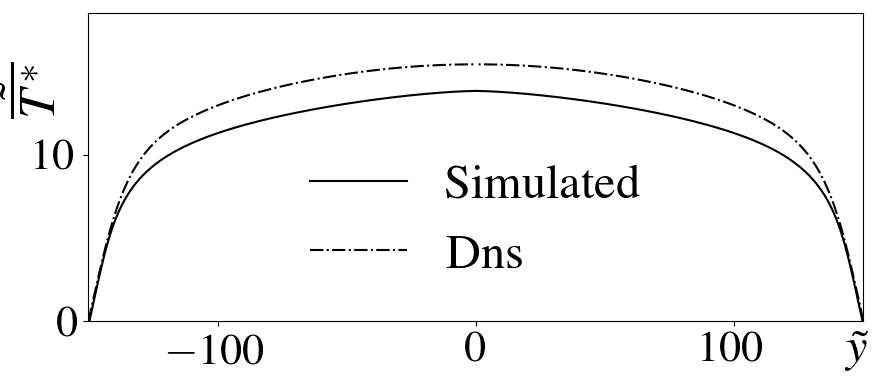
\includegraphics[angle=0, scale=0.20]{fotos_formatacao_final/Temperature_150_071_classico}
          \caption{$Re_\tau = 150$, $L2_t = 1.42$}
        \end{minipage}
        \hfill
        \begin{minipage}{0.49\textwidth}
          \centering
          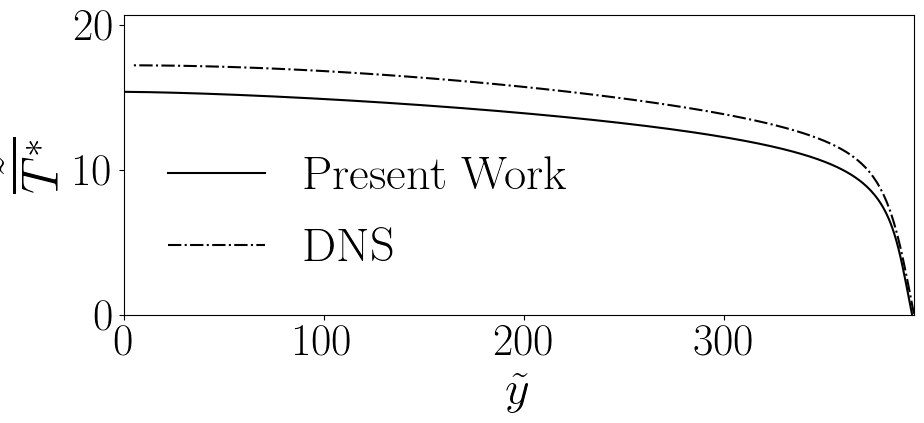
\includegraphics[angle=0, scale=0.20]{fotos_formatacao_final/Temperature_395_071_classico}
          \caption{$Re_\tau = 395$, $L2_t = 1.55$}
        \end{minipage}
        \begin{minipage}{0.49\textwidth}
          \centering
          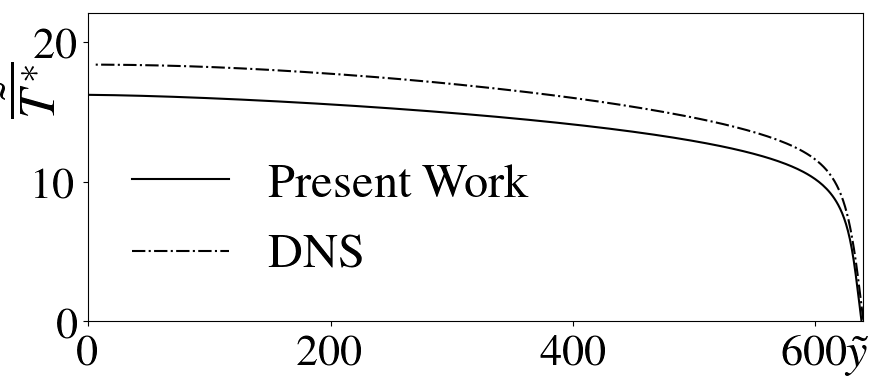
\includegraphics[angle=0, scale=0.20]{fotos_formatacao_final/Temperature_640_071_classico}
          \caption{$Re_\tau = 640$, $L2_t = 1.79$}
        \end{minipage}
        \hfill
        \begin{minipage}{0.49\textwidth}
          \centering
          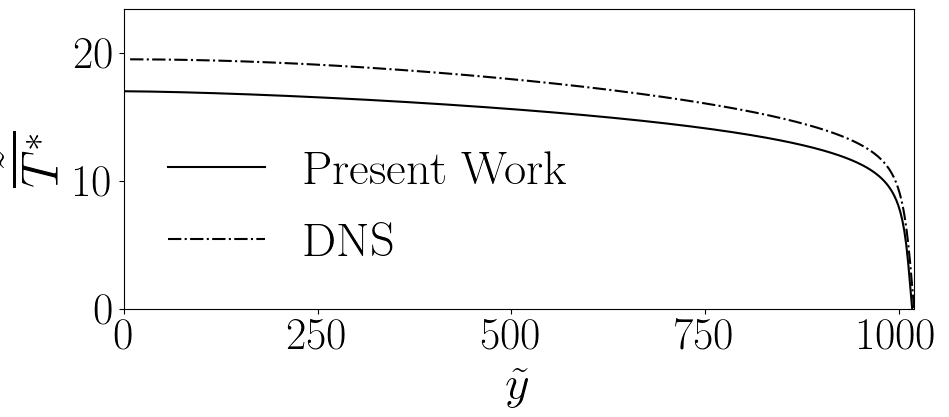
\includegraphics[angle=0, scale=0.20]{fotos_formatacao_final/Temperature_1000_071_classico}
          \caption{$Re_\tau = 1020$, $L2_t = 2.04$}
        \end{minipage}
        \caption{Distribuição de temperatura para $Pr_t = 0.71$ e $A = 26$.} 
        \label{figuraresultados1}
    \end{figure}
  \end{frame}
	
	
	
	
		
		\begin{frame}
		\frametitle{Estudo do número de Prandtl turbulento fornecido por DNS}
		\begin{minipage}[h!]{0.29\textwidth}
			$\bullet$ O número de Prandtl turbulento do DNS era diferente do que utilizamos ($0.71$).\\
      $\bullet$ O valor do número de Prandtl turbulento não só varia com o número de Reynolds e número de Prandtl, mas também com a distância até a parede.\\
      $\bullet$ Usando-se o valor de Prandtl turbulento fornecido pelo DNS obteve-se uma norma L2 de $0.19$ para $Re_t = 640$;
		\end{minipage}\hfill
		\begin{minipage}[h!]{0.60\textwidth}
      \begin{figure}[h!]
        \centering
        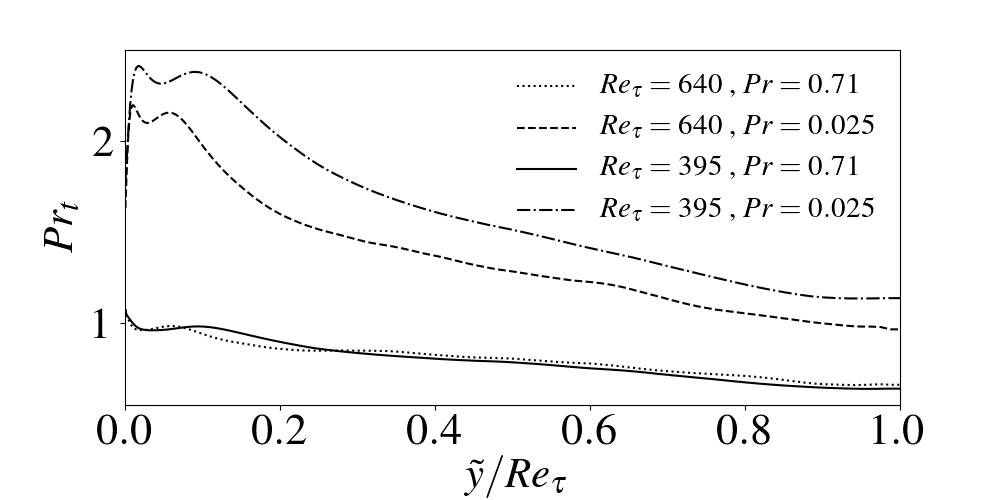
\includegraphics[angle=0, scale=0.39]{fotos_formatacao_final/DNS_PRt}
        \caption{Número de Prandtl turbulento adquirido do DNS em função de $ \tilde{y}/Re_\tau $, a distância até a parede no canal.}
        \label{figure5}
      \end{figure}
		\end{minipage}	\\
		\end{frame}
	
	
		\begin{frame}
		\frametitle{Ajustando o número de Prandtl turbulento com algoritmo genético}
		\begin{minipage}[h!]{0.39\textwidth}
      Foi utilizado um algoritmo de evolução diferencial na procura da melhor parametrização possível do Prandtl turbulento.

      $\bullet$ Arbitrou-se a norma L2 como função objetiva.\\
      $\bullet$ O número de Prandtl turbulento foi fornecido como única variável mutável.\\
      $\bullet$ As gerações se sucederam conforme o gráfico.\\

		\end{minipage}
    \begin{minipage}[h!]{0.60\textwidth}
      \begin{figure}[!h]
        \centering
        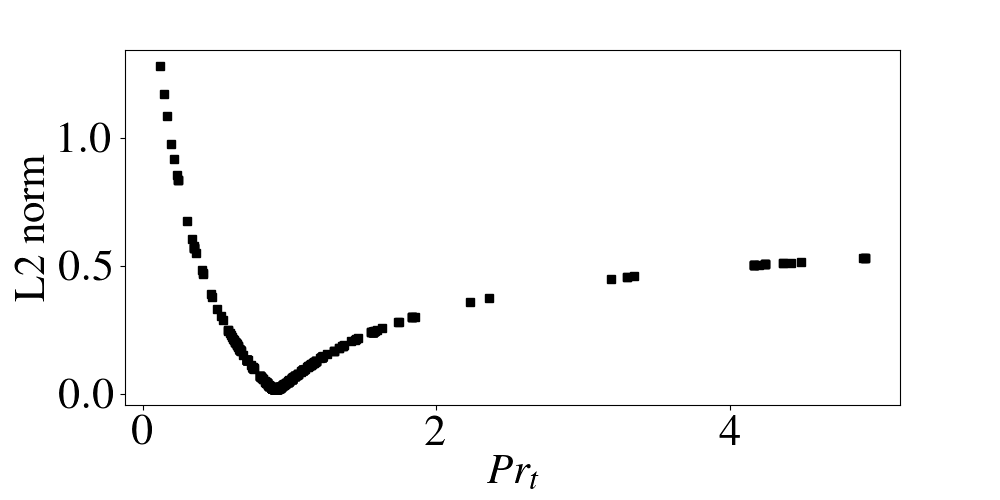
\includegraphics[angle=0, scale=0.41]{fotos_formatacao_final/Genetic_amostra}
        \caption{Iterações de algoritmo genético, com simulações para $Re_\tau = 1020$. Convergência em $Pr_t = 0.9 $.}
      \end{figure}
      \end{minipage}	
		\end{frame}
		

		\begin{frame}
		\frametitle{Resultados para: $Pr_t = 0.9$ , $A = 26$}
      \begin{figure}[!h]
        \centering
        \begin{minipage}[t]{0.49\textwidth}
          \centering
          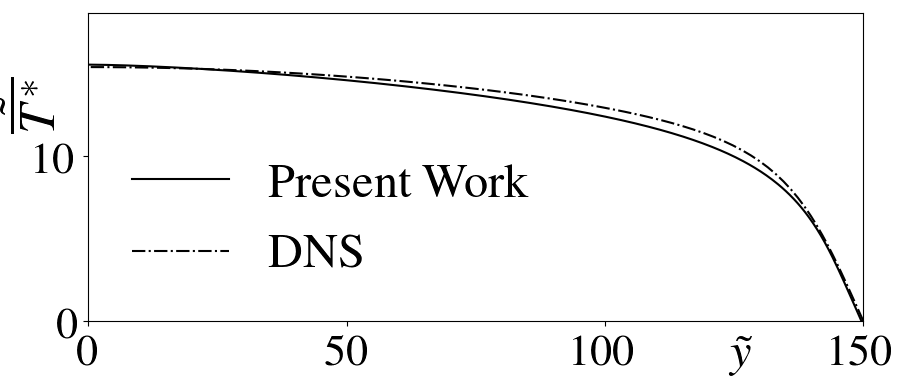
\includegraphics[angle=0, scale=0.2]{fotos_formatacao_final/Temperature_150_071_Prt0905_A26}
          \caption{$Re_\tau = 150$, $L2_t = 0.34$}
        \end{minipage}
        \begin{minipage}[t]{0.49\textwidth}
          \centering
          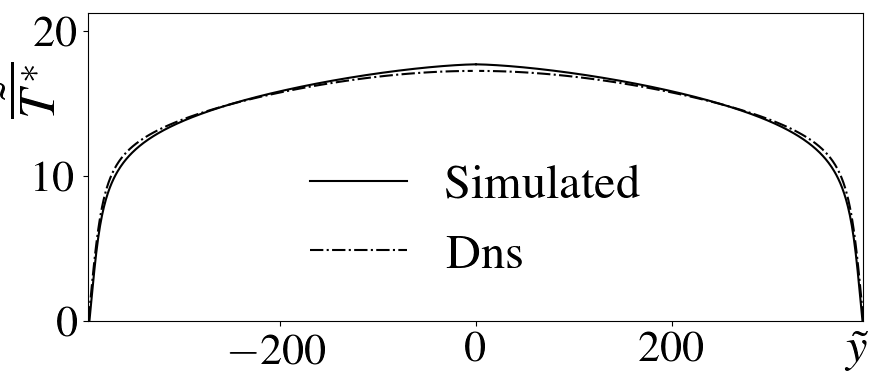
\includegraphics[angle=0, scale=0.2]{fotos_formatacao_final/Temperature_395_071_Prt0905_A26}
          \caption{$Re_\tau = 395$, $L2_t = 0.23$}
        \end{minipage}
        \begin{minipage}[t]{0.49\textwidth}
          \centering
          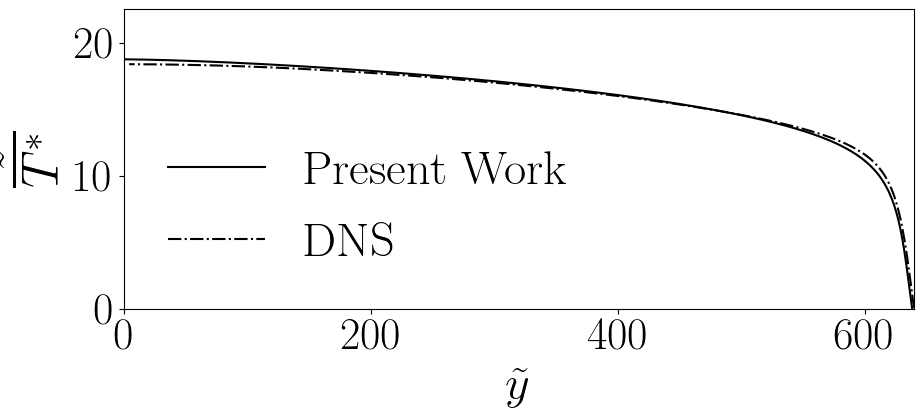
\includegraphics[angle=0, scale=0.2]{fotos_formatacao_final/Temperature_640_071_Prt0905_A26}
          \caption{$Re_\tau = 640$, $L2_t = 0.19$}
        \end{minipage}
        \begin{minipage}[t]{0.49\textwidth}
          \centering
          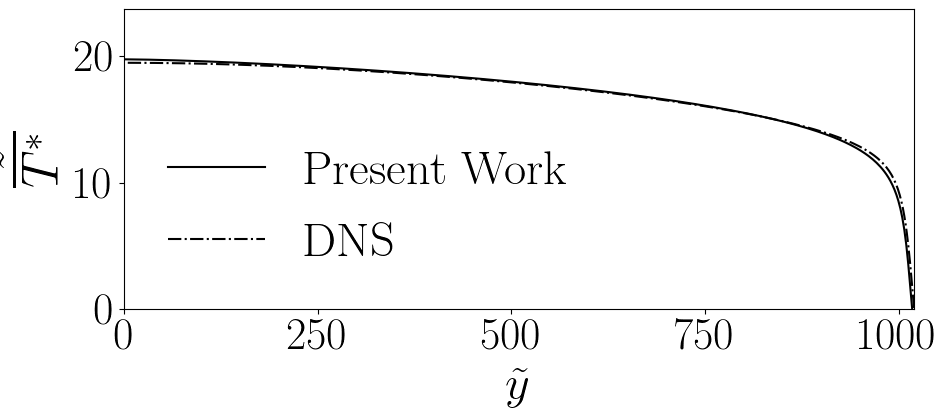
\includegraphics[angle=0, scale=0.2]{fotos_formatacao_final/Temperature_1000_071_Prt0905_A26}
          \caption{$Re_\tau = 1020$, $L2_t = 0.14$}
        \end{minipage}	
        \caption{Perfis de temperatura para simulações com $Pr_t = 0.9 $ e $A = 26$.}
        \label{primeiros}
      \end{figure}
		\end{frame}	
	
	
	
	
		
		\begin{frame}
		\frametitle{Algoritmo de otimização}
    Foi observado que o número de Prandtl turbulento varia com o número de Reynolds, logo, o mesmo processo foi feito para cada valor de Reynolds.\\

      Os valores obtidos podem ser conferidos na tabela \ref{tabela1}:

      \begin{table}[!h]
        \centering
        \caption{Números de prandtl turbulentos ideais ajustados para cada número de Reynolds turbulento, com a constante de cebeci $A = 26$.}
        \begin{tabular}{ll}
            \hline
            $Re_\tau$ & $Pr_t$\\
            \hline
            150  &   0.94531\\
            395  &   0.89531\\
            640  &   0.89531\\
            1020 &   0.90000\\ 
            \hline
        \end{tabular}
        \label{tabela1}
      \end{table}
		\end{frame}	
	
	
	
	
		\begin{frame}
		\frametitle{Ajuste dos valores obtidos}
			$\bullet$ Executando um ajuste de curva polinomial, obteve-se a seguinte relação:
      \begin{equation}
        \begin{split}
          Pr_t = -4.5604 * 10^{-10} Re_\tau^3 + 9.5690 * 10^{-7} Re_\tau^2\\
          - 6.1715 *10 ^{-4} Re_\tau + 1.0178 .
        \end{split}
      \end{equation}
			Assim, desenvolveu-se um modelo ajustado para o número de Prandtl turbulento em função do número de Reynolds turbulento.
		\end{frame}	


    \begin{frame}
		\frametitle{Resultados para: $Pr_t(Re_\tau)$, $A = 26$}
    \begin{figure}[!h]
        \centering
        \begin{minipage}[t]{0.5\textwidth}
          \centering
          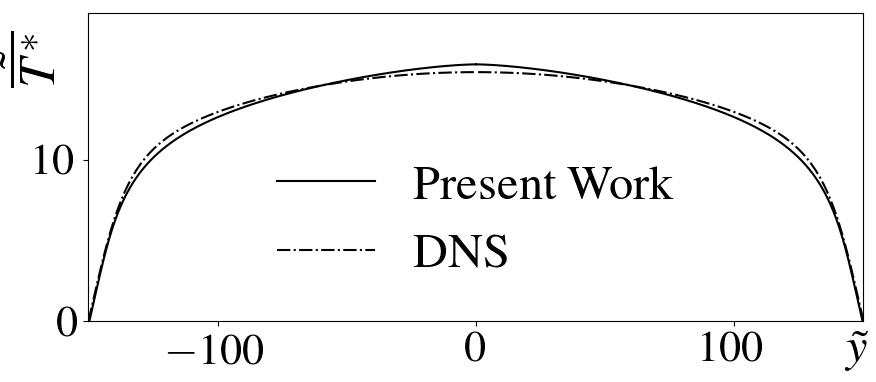
\includegraphics[angle=0, scale=0.2]{fotos_formatacao_final/Temperature_150_071_Prt(Ret)_A26}
          \caption{$Re_\tau = 150$, $L2_t = 0.26$}
        \end{minipage}
        \begin{minipage}[t]{0.45\textwidth}
          \centering
          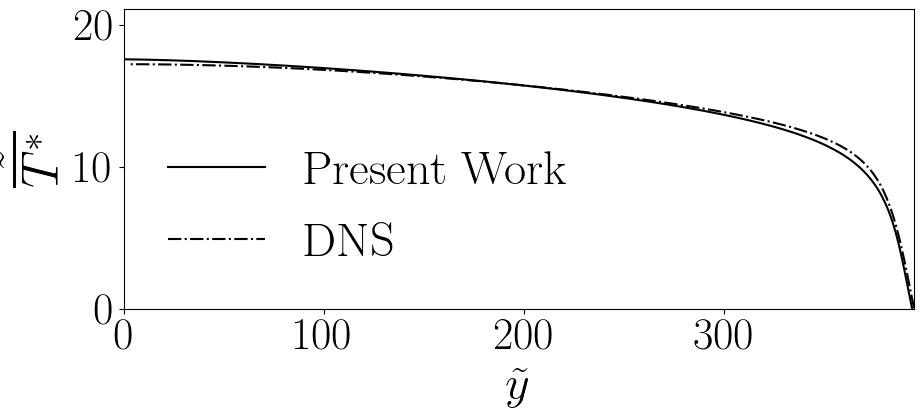
\includegraphics[angle=0, scale=0.2]{fotos_formatacao_final/Temperature_395_071_Prt(Ret)_A26}
          \caption{$Re_\tau = 395$, $L2_t = 0.22$}
        \end{minipage}
        \begin{minipage}[t]{0.5\textwidth}
          \centering
          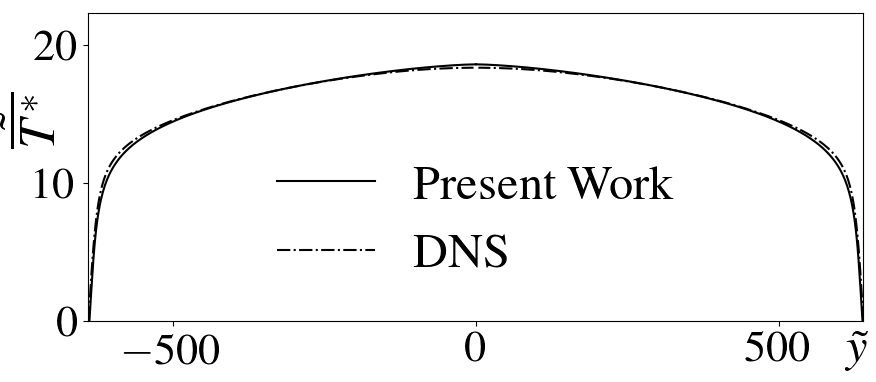
\includegraphics[angle=0, scale=0.2]{fotos_formatacao_final/Temperature_640_071_Prt(Ret)_A26}
          \caption{$Re_\tau = 640$, $L2_t = 0.17$}
        \end{minipage}
        \begin{minipage}[t]{0.45\textwidth}
          \centering
          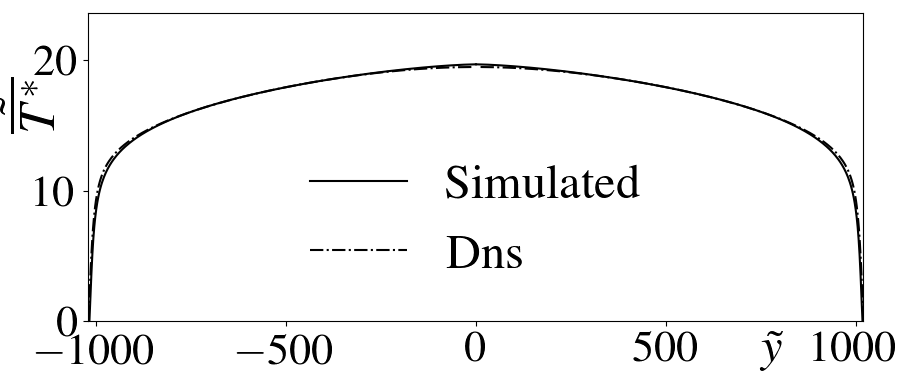
\includegraphics[angle=0, scale=0.2]{fotos_formatacao_final/Temperature_1000_071_Prt(Ret)_A26}
          \caption{$Re_\tau = 1020$, $L2_t = 0.14$}
        \end{minipage}	
        \caption{Resultados de temperatura para $Pr_\tau(Re_\tau)$, $A = 26$ e $Pr =0.71$. }
        \label{figura_9}
      \end{figure}

		\end{frame}	


    \begin{frame}
		\frametitle{Análise sobre o perfil dinâmico}
      \begin{figure}[!h]
        \centering
        \begin{minipage}[t]{0.5\textwidth}
          \centering
          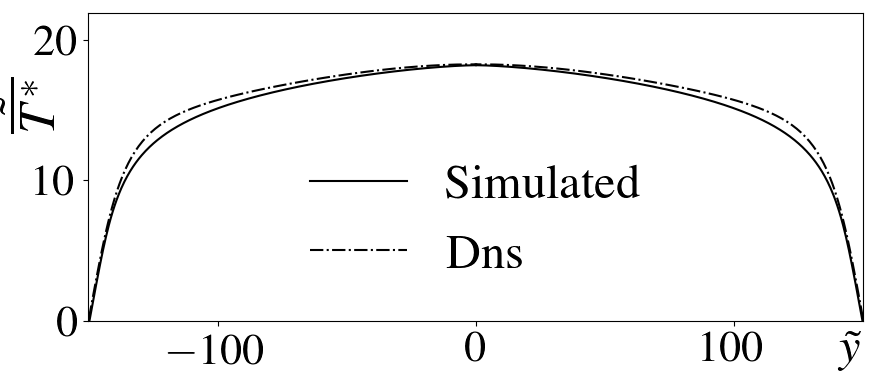
\includegraphics[angle=0, scale=0.2]{fotos_formatacao_final/Temperature_150_Avelocity}
          \caption{$Re_\tau = 150$, $L2_d = 0.47$}
        \end{minipage}
        \begin{minipage}[t]{0.45\textwidth}
          \centering
          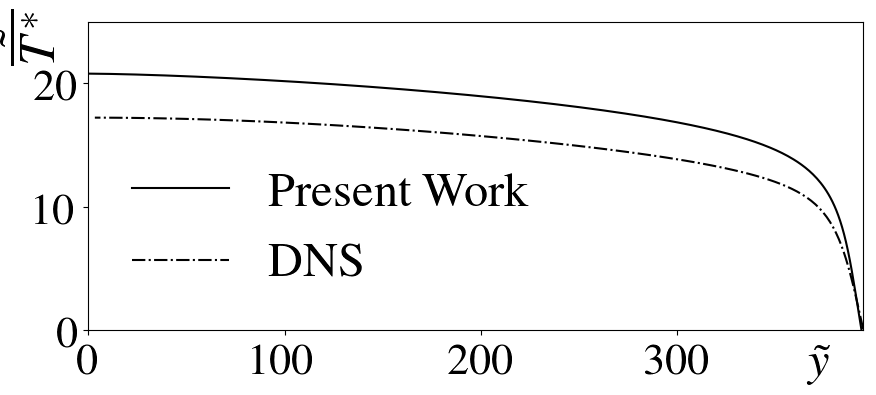
\includegraphics[angle=0, scale=0.2]{fotos_formatacao_final/Temperature_395_Avelocity}
          \caption{$Re_\tau = 395$, $L2_d = 0.17$}
        \end{minipage}
        \begin{minipage}[t]{0.5\textwidth}
          \centering
          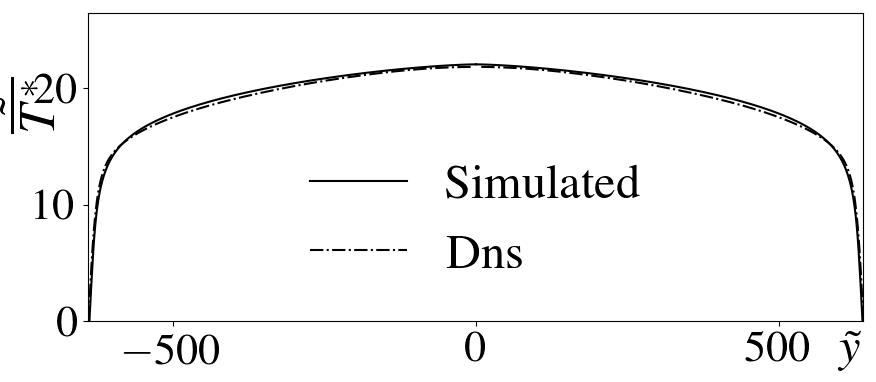
\includegraphics[angle=0, scale=0.2]{fotos_formatacao_final/Temperature_640_Avelocity}
          \caption{$Re_\tau = 640$, $L2_d = 0.23$}
        \end{minipage}
        \begin{minipage}[t]{0.45\textwidth}
          \centering
          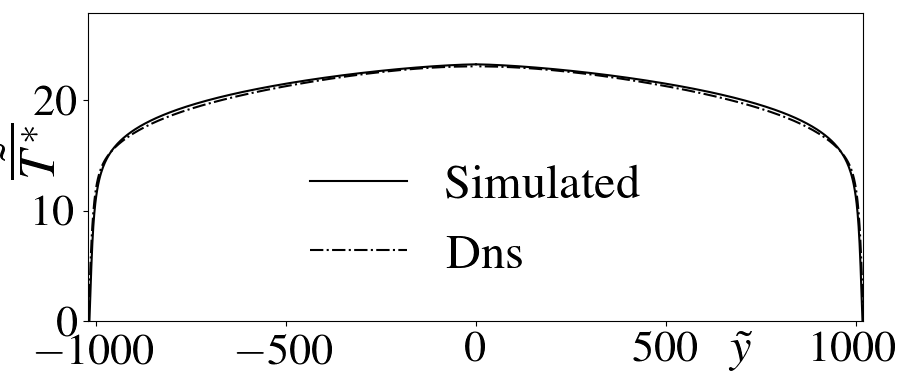
\includegraphics[angle=0, scale=0.2]{fotos_formatacao_final/Temperature_1000_Avelocity}
          \caption{$Re_\tau = 1020$, $L2_d = 0.23$}
        \end{minipage}	
        \caption{Resultados de perfil de velocidade para $A = 26$.}
        \label{figura_10}
      \end{figure}
		\end{frame}	
		
		
	
	
		\begin{frame}
		\frametitle{Ajuste do valor de Cebeci}
		\begin{minipage}[h!]{0.45\textwidth}
      O valor da constate de Cebeci foi ajustada da mesma forma como foi feito com o Prandtl turbulento.
			A partir dos pontos resultantes do algoritmo de otimização, se desenvolveu o modelo ajustado para o valor de Cebeci. Como segue:
			\begin{equation}
			A = \frac{Re_\tau ^{0.0451 * \ln(Re_\tau)} *e ^ {5.2753} }{Re_\tau ^{0.6094}}
			\end{equation}
		\end{minipage}\hfill
		\begin{minipage}[h!]{0.45\textwidth}
    \begin{table}[!h]
	\centering
	\caption{Constante de Cebeci ideal ajustada para cada número de Reynolds turbulento.}
	\begin{tabular}{ll}
		\hline
		$Re_\tau$ & $A$\\
		\hline
		150  &   28.616180\\
		395  &   25.673782\\
		640  &   25.001266\\
		1020 &   25.002136\\ 
		\hline
	\end{tabular}
	\label{tablea}
\end{table}


		\end{minipage}
		\end{frame}	


    \begin{frame}
		\frametitle{Resultados para: $A(Re_\tau)$}
\begin{figure}[!h]
	\centering
	\begin{minipage}[t]{0.5\textwidth}
		\centering
		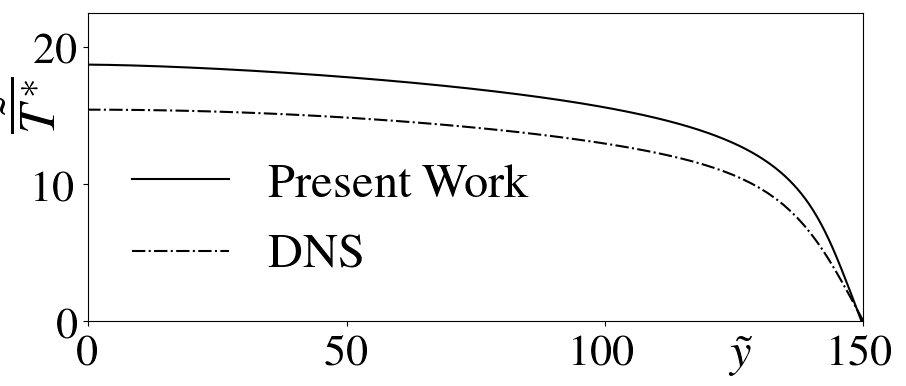
\includegraphics[angle=0, scale=0.2]{fotos_formatacao_final/Temperature_150_Amodeled}
		\caption{$Re_\tau = 150$, $L2_d = 0.28$}
	\end{minipage}
	\begin{minipage}[t]{0.45\textwidth}
		\centering
		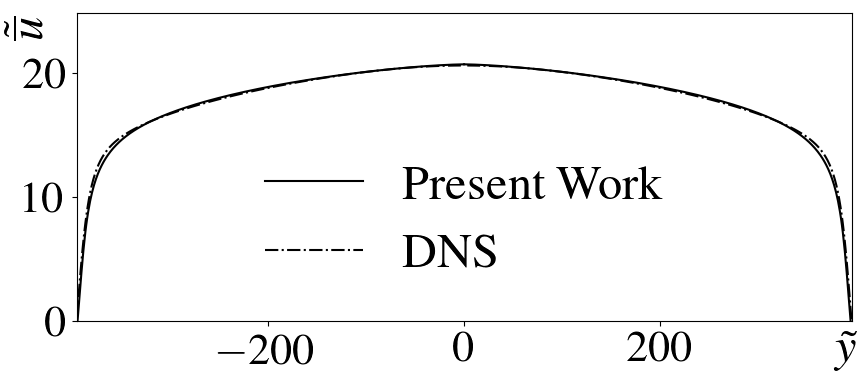
\includegraphics[angle=0, scale=0.2]{fotos_formatacao_final/Temperature_395_Amodeled}
		\caption{$Re_\tau = 395$, $L2_d = 0.16$}
	\end{minipage}
	\begin{minipage}[t]{0.5\textwidth}
		\centering
		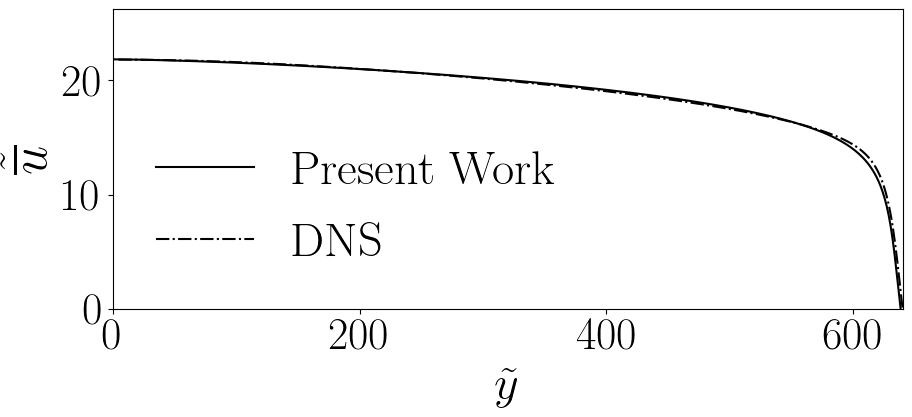
\includegraphics[angle=0, scale=0.2]{fotos_formatacao_final/Temperature_640_Amodeled}
		\caption{$Re_\tau = 640$, $L2_d = 0.14$}
	\end{minipage}
	\begin{minipage}[t]{0.45\textwidth}
		\centering
		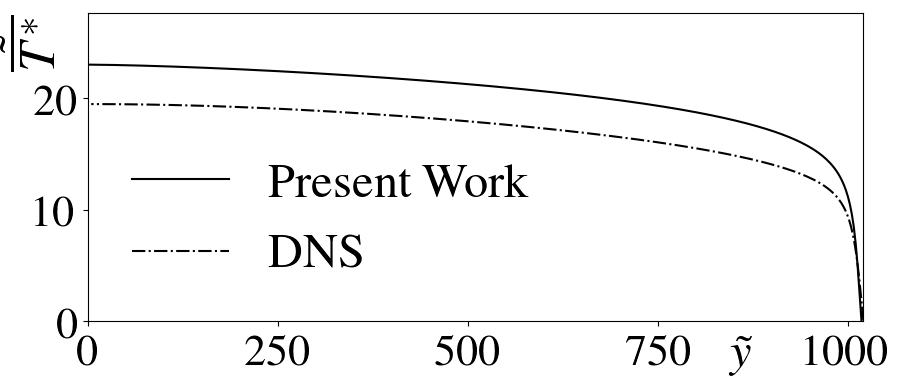
\includegraphics[angle=0, scale=0.2]{fotos_formatacao_final/Temperature_1000_Amodeled}
		\caption{$Re_\tau = 1020$, $L2_d = 0.13$}
	\end{minipage}	
	\caption{Resultados em distribuição de velocidade para o modelo de A.}
\end{figure}
		\end{frame}	

	
	
    \begin{frame}
		\frametitle{Análise sobre o perfil dinâmico}
		\begin{minipage}[h!]{0.45\textwidth}
      $\bullet$ Com o modelo de Cebeci ajustado novos valores de Prandtl turbulento foram calculados com o algoritmo genético.\\
      $\bullet$ A partir dos novos valores numéricos, um novo modelo foi desenvolvido:\\

      \begin{equation}
        \begin{split}
          Pr_t = 4.5290 * 10^{-12} Re_\tau^3 \\
          - 5.7395 * 10^{-8} Re_\tau^2 + 9.397 * 10^{-5} Re_\tau + 0.8731.
        \end{split}
      \end{equation}

		\end{minipage}\hfill
		\begin{minipage}[h!]{0.45\textwidth}
      \begin{table}[!h]
        \centering
        \caption{Números de prandtl turbulentos ideais ajustados para cada número de Reynolds turbulento, com a função de Cebeci ajustada.}
        \begin{tabular}{ll}
          \hline
          $Re_\tau$ & $Pr_t$\\
          \hline
          150  &   0.88594\\
          395  &   0.90156\\
          640  &   0.91094\\
          1020 &   0.91406\\ 
          \hline
        \end{tabular}
      \end{table}

		\end{minipage}
		\end{frame}	


    \begin{frame}
		\frametitle{Resultados para: $Pr_\tau(Re_\tau)$, $A(Re_\tau)$}
      \begin{figure}[!h]
        \centering
        \begin{minipage}[t]{0.5\textwidth}
          \centering
          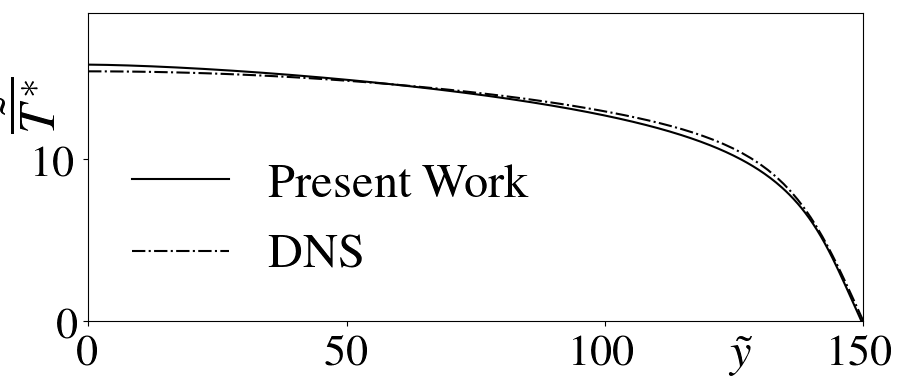
\includegraphics[angle=0, scale=0.2]{fotos_formatacao_final/Temperature_150_071_Prt(Ret)_Avelocity}
          \caption{$Re_\tau = 150$, $L2_t = 0.212$}
        \end{minipage}
        \begin{minipage}[t]{0.45\textwidth}
          \centering
          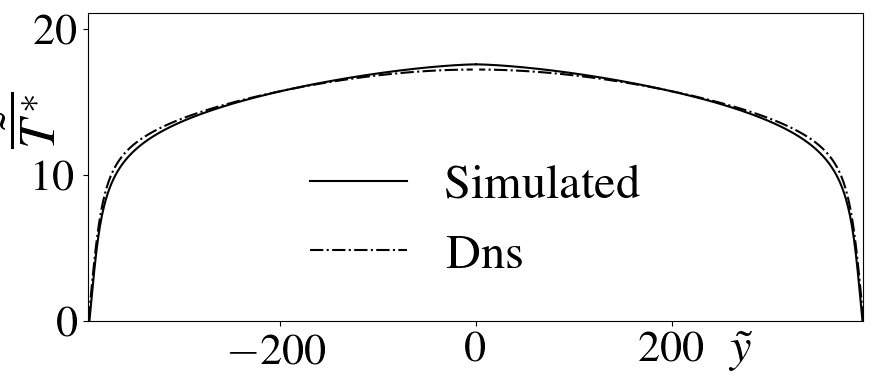
\includegraphics[angle=0, scale=0.2]{fotos_formatacao_final/Temperature_395_071_Prt(Ret)_Avelocity}
          \caption{$Re_\tau = 395$, $L2_t = 0.233$}
        \end{minipage}
        \begin{minipage}[t]{0.5\textwidth}
          \centering
          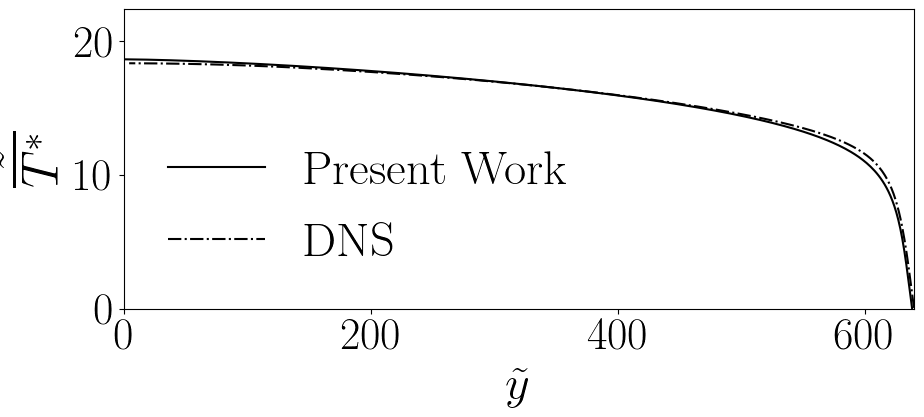
\includegraphics[angle=0, scale=0.2]{fotos_formatacao_final/Temperature_640_071_Prt(Ret)_Avelocity}
          \caption{$Re_\tau = 640$, $L2_t = 0.205$}
        \end{minipage}
        \begin{minipage}[t]{0.45\textwidth}
          \centering
          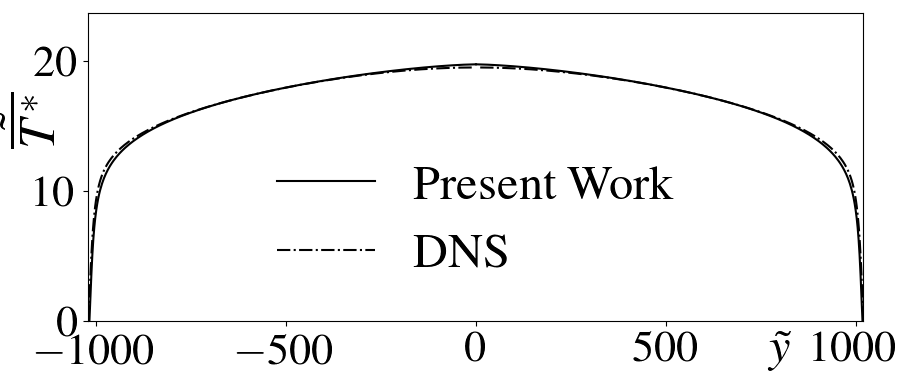
\includegraphics[angle=0, scale=0.2]{fotos_formatacao_final/Temperature_1000_071_Prt(Ret)_Avelocity}
          \caption{$Re_\tau = 1020$, $L2_t = 0.175$}
        \end{minipage}	
        \caption{Resultados térmicos para $Pr_\tau(Re\tau)$, $A(Re_\tau)$ e $Pr =0.71$ }
      \end{figure}
		\end{frame}

    \begin{frame}
		\frametitle{Ajuste multiobjetivo}
		\begin{minipage}[h!]{0.45\textwidth}
      $\bullet$ Um novo modelo foi criado considerando o Prandtl turbulento, e a constante de cebeci para os casos térmico e dinâmico como variáveis editáveis.
      \begin{equation}
        A_t = \frac{Re_\tau ^{0.0395 \ln(Re_\tau)^2 - 0.7588 \ln(Re_\tau) +  4.6637  } }{e ^{5.6703}},
      \end{equation}

      \begin{equation}
        \begin{split}
          Pr_t = -2.4892 * 10^{-10} Re_\tau^3 +  3.6036 * 10^{-7} Re_\tau^2\\
          + 3.7921 *10 ^{-5} Re_\tau + 0.7123 .
        \end{split}
      \end{equation}

		\end{minipage}\hfill
		\begin{minipage}[h!]{0.45\textwidth}
      \begin{table}[!h]
        \centering
        \caption{Números de prandtl turbulentos ideais e função de cebeci térmica ($A_t$) ajustados para cada número de Reynolds turbulento, com a abordagem multiobjetiva.}
        \begin{tabular}{llll}
          \hline
          $Re_\tau$ & $Pr_t$ & $A_t$ & $A_d$\\
          \hline
          150  &   0.72530 & 37.25510 & 28.616180\\
          395  &   0.76821 & 34.24176 & 25.673782\\
          640  &   0.81896 & 31.27627 & 25.001266\\
          1020 &   0.86179 & 28.73726 & 25.002136\\ 
          \hline
        \end{tabular}
      \end{table}
		\end{minipage}
		\end{frame}
	
	
    \begin{frame}
		\frametitle{Resultados para: $Pr_\tau(Re_\tau)$, $A_t(Re_\tau)$, $A_d(Re_\tau)$}
    \begin{figure}[!h]
        \centering
        \begin{minipage}[t]{0.5\textwidth}
          \centering
          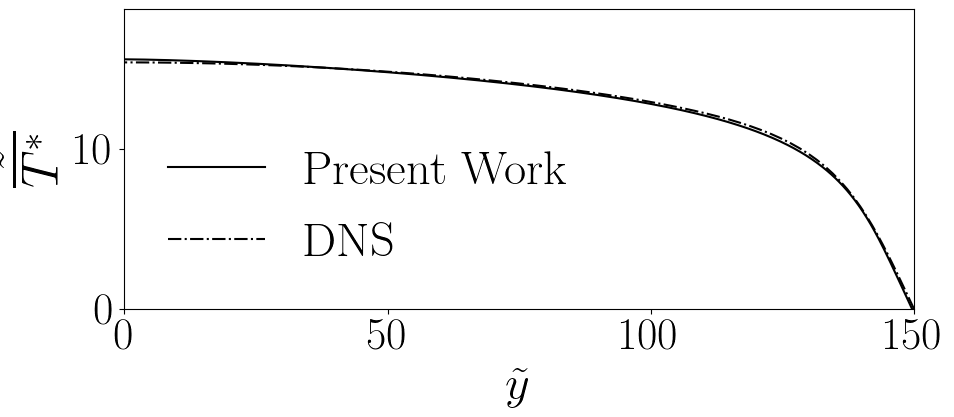
\includegraphics[angle=0, scale=0.2]{fotos_formatacao_final/Temperature_150_071_Genetic2temperature}
          \caption{$Re_\tau = 150$, $L2_t = 0.091$}
        \end{minipage}
        \begin{minipage}[t]{0.45\textwidth}
          \centering
          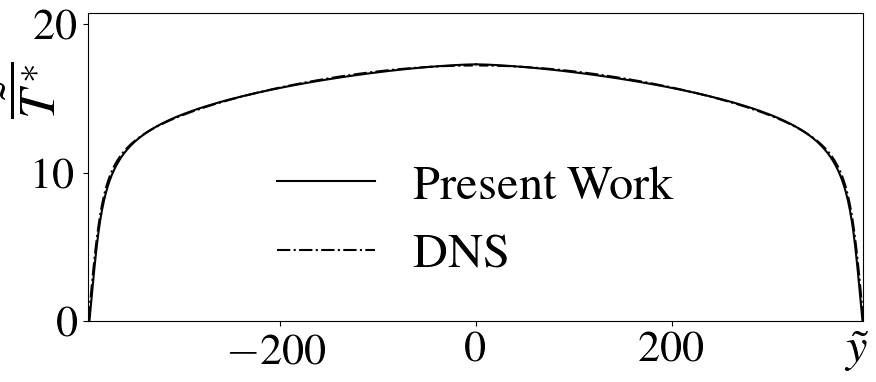
\includegraphics[angle=0, scale=0.2]{fotos_formatacao_final/Temperature_395_071_Genetic2temperature}
          \caption{$Re_\tau = 395$, $L2_t = 0.049$}
        \end{minipage}
        \begin{minipage}[t]{0.5\textwidth}
          \centering
          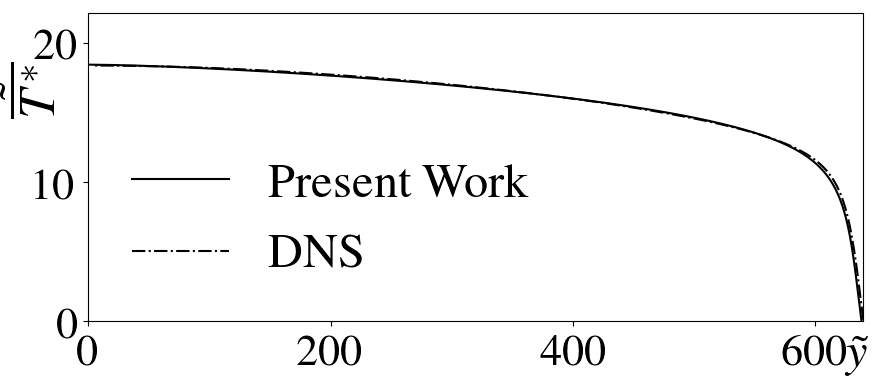
\includegraphics[angle=0, scale=0.2]{fotos_formatacao_final/Temperature_640_071_Genetic2temperature}
          \caption{$Re_\tau = 640$, $L2_t = 0.061$}
        \end{minipage}
        \begin{minipage}[t]{0.45\textwidth}
          \centering
          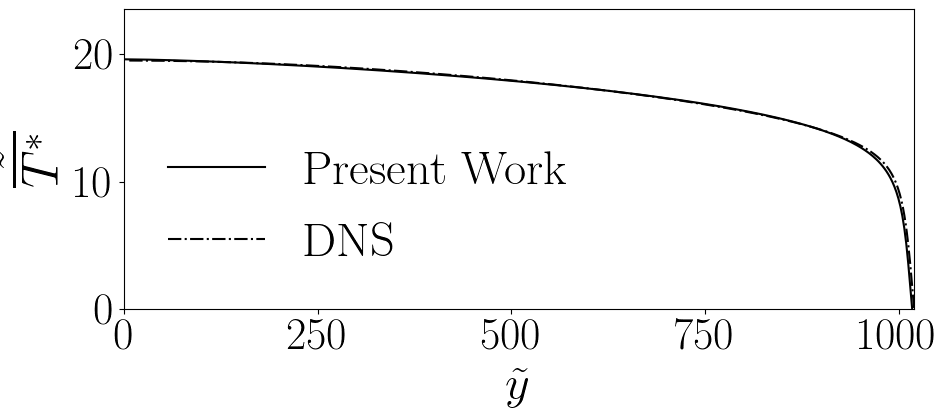
\includegraphics[angle=0, scale=0.2]{fotos_formatacao_final/Temperature_1000_071_Genetic2temperature}
          \caption{$Re_\tau = 1020$, $L2_t = 0.076$}
        \end{minipage}	
        \caption{Resultados de simulação térmica para $Pr_\tau(Re_\tau)$, $A_d(Re_\tau)$, $A_t(Re_\tau) $ e $Pr =0.71$,\\ com ajuste multiobjetivo.}
      \end{figure}
		\end{frame}	
	
	\section{Conclusão}

  \begin{frame}
    \frametitle{Conclusão}
    \begin{itemize}
      \item O método semi analítico para o campo de temperatura foi implementado com sucesso e validado com os dados de DNS. Os resultados foram satisfatórios.
      \item A investigação sobre o número de Prandtl turbulento e a constante de Cebeci se mostrou muito instrutiva ao descrever como estas constantes ajustadas podem influenciar no resultado do método semi-analítico.
      \item Ajustando-se o valor do número de Prandtl turbulento e da constante de Cebeci com algoritmos genéticos resultou em erros cada vez menores, mas com sobre encaixe, o que torna tais valores úteis somente para o modelo físico explorado no presente trabalho.
      \item Apesar disso, encontrou-se valores muito melhores que os inicialmente usados, com resultados muito mais acurados.
    \end{itemize}
  \end{frame}
	
	
	
	
	
	\section{Agradecimentos}
		
		
		
		
		
			\begin{frame}
				\placelogomflab 
				\frametitle{Agradecimentos}
				\begin{figure}
					\begin{center}
						\begin{tabular}{c c}
							{
\includegraphics[trim=0.0cm 0.0cm 0.0cm 0.0cm,clip=true,height=0.2\textheight]{figuras/petrobras.png}}&{
\includegraphics[trim=0.0cm 0.0cm 0.0cm 0.0cm,clip=true,height=0.2\textheight]{figuras/logo_mflab.png}}\\
							{
\includegraphics[trim=0.0cm 0.0cm 0.0cm 0.0cm,clip=true,height=0.2\textheight]{figuras/cnpq.png}}&{
\includegraphics[trim=0.0cm 0.0cm 0.0cm 0.0cm,clip=true,height=0.2\textheight]{figuras/CAPES.png}}\\
							{
\includegraphics[trim=0.0cm 0.0cm 0.0cm 0.0cm,clip=true,height=0.2\textheight]{figuras/FAPEMIG.jpg}}&{
\includegraphics[trim=0.0cm 0.0cm 0.0cm 0.0cm,clip=true,height=0.2\textheight]{figuras/UFU_black.jpg}}\\
						\end{tabular}
					\end{center}
				\end{figure}
			\end{frame}
			
			
			
			
			
			\begin{frame}
				\placelogomflab 
				\frametitle{Agradecimentos}
				\fontsize{44pt}{7.2}\selectfont
				\begin{center}
					Obrigado.\\
				\fontsize{20pt}{7.2}\selectfont
          Perguntas?
				\end{center}
			\end{frame}
		
		
		
		
\end{document}




		



%%%%%%%%%%%%%%%%%%%%%%%%%%%%%%%%%%%%%%% Exemplo de formatação de imagens		
%		\begin{frame}
%			\frametitle{Adição de fronteiras extras}
%			\begin{tabular}{c c}
%				
%				{\includegraphics[trim=0.0cm 0.0cm 0.0cm 0.0cm,clip=true,loop,height=0.5\textheight]{figuras/filtration_depois.png}}&{\includegraphics[trim=0.0cm 0.0cm 0.0cm 0.0cm,clip=true,loop,height=0.4\textheight]{figuras/filtration_depois_zoom.png}}\\
%				
%			\end{tabular}
%			
%		\end{frame}




%%%%%%%%%%%%%%%%%%%%%%%%%%%%%%%%%%%%%% Exemplo de formatação de imagens		
%		\begin{frame}
%			\frametitle{Agora}
%			\centering
%			\begin{tabular}{c}
%				
%				{\includegraphics[trim=0.00cm 2.0cm 0.0cm 2.0cm,clip=true,loop,width=0.9\textwidth]{figuras/t_x_51f.png}}\\{\includegraphics[trim=0.01cm 0.0cm 0.01cm 0.0cm,clip=true,loop,width=0.9\textwidth]{figuras/t_x_51999.png}}\\{\includegraphics[trim=0.01cm 0.0cm 0.01cm 0.0cm,clip=true,loop,width=0.9\textwidth]{figuras/t_x_51999g.png}}\\{\includegraphics[trim=0.01cm 0.0cm 0.01cm 0.0cm,clip=true,loop,width=0.9\textwidth]{figuras/t_x_51999y.png}}\\{\includegraphics[trim=0.01cm 0.0cm 0.01cm 0.0cm,clip=true,loop,width=0.9\textwidth]{figuras/t_x_51999b.png}}
%				
%			\end{tabular}
%			
%		\end{frame}





%%%%%%%%%%%%%%%%%%%%%%%%%%%%%%%%%%%%%  Formatação de equações:		
%		\begin{frame}
%			\frametitle{Newton-Raphson}
%			
%			\flushleft
%			Método de interface com jacobiano composto:
%			
%			\centering
%			\begin{equation}\label{forte_eqNewton}
%			K(D+\Delta D) \approx K(D)+\Delta D \, J(D)
%			\end{equation}
%			\begin{equation}\label{forte_eqNewton2}
%			K(D) =  Estrutura(Fluido(D))-D =  0
%			\end{equation}
%			\begin{equation}\label{forte_eqNewton3}
%			J(D) =  Estrutura'(Fluido(D)) \, Fluido'(D)-I
%			\end{equation}
%			\begin{equation}\label{forte_eqNewton4}
%			Fluido(D): \mathbb{R}^{n} \to \mathbb{R}^{m}
%			\end{equation}
%			
%			\flushleft
%			$Fluido'(D)$ é de tamanho $m x n$
%			
%			\centering
%			
%			\begin{equation}\label{forte_eqNewton5}
%			Estrutura(F): \mathbb{R}^{m} \to \mathbb{R}^{n}
%			\end{equation}
%			
%			\flushleft
%			$Estrutura'(F)$ é de tamanho $n x m$\\
%			$Estrutura'(Fluido(D)) \, Fluido'(D)$ e $I$ é de tamanho $n x n$
%		\end{frame}




%%%%%%%%%%%%%%%%%%%%%%%%%%%%%%%%%%%%%%%%%%% Vários exemplos de formatação textual:		


%		\begin{frame}
%			\frametitle{Conveniência do método de Multi Direct Forcing}
%			
%			\flushleft
%			\textbf{Fraco:}\\
%			$\bullet$ Predição da velocidade.\\
%			$\bullet$ MDF. (Imposição da condição de dirichlet na interface e cálculo da força)\\
%			$\bullet$ Estrutura.\\
%			$\bullet$ Poisson.\\
%			$\bullet$ Correção de velocidade e pressão.\\ \\
%
%			\textbf{Forte:}\\
%			$\bullet$ Predição da velocidade.\\
%			while \\
%			\quad	$\longrightarrow$ MDF.\\
%			\quad	$\longrightarrow$ Estrutura.\\
%			end\\
%			$\bullet$ Poisson.\\
%			$\bullet$ Correção de velocidade e pressão.\\
%
%		\end{frame}

		

%		
%%%%%%%%%%%%%%%%%%%%%%%%%%%%%%%%%  Modelo duas fotos lado a lado:


%		\begin{frame}
%		\frametitle{Limite do fraco}
%			ct=121
%			mi=200
%			\begin{tabular}{c c}
%			{\includegraphics[width=0.45\linewidth]{../../simulacoes_Estudo_dirigido2/fraco_mi_200_0_15_ct141/figuras/estrutura/vel_151}}&
%		   {\includegraphics[width=0.45\linewidth]{../../simulacoes_Estudo_dirigido2/fraco_mi_200_0_15_ct141/figuras/estrutura/vel_251}}\\
%		   {(a) Velocidade em linha centro da estrutura} & {(b) Velocidade transversal centro da estrutura}
%		\end{tabular}
%		\end{frame}



%%%%%%%%%%%%%%%%%%%%%%%%%%%%%%%%%%  Modelo tabela :

%		\begin{frame}
%			\frametitle{Comparação número de iterações}
%			\begin{tabular}{c c c c}
%				\hline
%				Método & Mínimo     &    Máximo &  Média\\ \hline
%				FPI MDF variável & 8     &    101 &  8.9764764764764760\\
%				FPI MDF fixo & 8     &     11 &  8.9099099099099099\\
%				QN Primeiro método de Broyden MDF variável & 18    &     101 &  18.281281281281281 \\ \hline
%			\end{tabular}
%		\end{frame}	




